%  LaTeX support: latex@mdpi.com
%  CIFA manuscript for Electronics (MDPI)
%  Compile with pdfLaTeX twice

%=================================================================
\documentclass[electronics,article,submit,moreauthors]{Definitions/mdpi}

%=================================================================
% MDPI internal commands - do not modify
\firstpage{1}
\makeatletter
\setcounter{page}{\@firstpage}
\makeatother
\pubvolume{1}
\issuenum{1}
\articlenumber{0}
\pubyear{2026}
\copyrightyear{2026}
\datereceived{ }
\daterevised{ }
\dateaccepted{ }
\datepublished{ }

%=================================================================
% Additional packages
\usepackage{amsmath,amssymb}
\usepackage{booktabs}
\usepackage{longtable}
\usepackage{graphicx}
\usepackage{url}

%=================================================================
% Tracked changes for the first revision: additions in blue, deletions
% in red with strike-through.
\usepackage{xcolor}
\usepackage{soul}
\usepackage{cancel}
% Algorithm float (R2-2): present the procedure as Algorithm 1 rather than as
% a table. The float package is already loaded by Definitions/mdpi.cls.
\floatstyle{plaintop}
\newfloat{algfloat}{t}{loa}
\floatname{algfloat}{Algorithm}
\definecolor{addblue}{RGB}{0,0,180}
\definecolor{delred}{RGB}{180,0,0}
\setstcolor{delred}
% Deletion of a citation: red strike-through over an mbox so that the
% citation internals are not parsed by soul.
\newcommand{\delcite}[1]{\textcolor{delred}{\sout{\mbox{\citep{#1}}}}}
% \add{...}    = newly inserted text (blue)
% \del{...}    = removed text (red with strike-through; text mode only)
% \delmath{...}= removed display/inline math (red with a cancel slash)
\newcommand{\add}[1]{\textcolor{addblue}{#1}}
\newcommand{\del}[1]{\textcolor{delred}{\st{#1}}}
\newcommand{\delmath}[1]{\textcolor{delred}{\cancel{#1}}}

% The abstract is passed to hyperref's pdfsubject inside \maketitle
% (Definitions/mdpi.cls), whose PDF-string context cannot typeset
% soul/color/cancel. Register the plain-text fallbacks after hyperref loads
% (it is loaded in a begindocument hook) but before \maketitle runs.
\AtBeginDocument{%
  \pdfstringdefDisableCommands{%
    \def\add#1{#1}%
    \def\del#1{}%
    \def\delmath#1{}%
    \def\delcite#1{}%
  }%
}

%=================================================================
% CLEAN VERSION: accept all tracked changes (no colors, no strikeout)
\makeatletter
\renewcommand{\add}[1]{#1}
\renewcommand{\del}[1]{}
\renewcommand{\delmath}[1]{}
\renewcommand{\delcite}[1]{}
\makeatother
%=================================================================
% Full title of the paper
\Title{Content-Conditioned Invariant Feature-Statistic Augmentation: Unifying Robustness and Weight Averaging for Domain Generalization}

% Author Orchid ID
\newcommand{\orcidauthorA}{0009-0006-0767-0842}

% Authors
\Author{Qingsong~Cai $^{1,*}$\orcidA{}, Hao~Wang $^{1}$ and Tianze~Hao $^{1}$}

% Authors for metadata
\AuthorNames{Qingsong Cai, Hao Wang and Tianze Hao}

% Affiliations
\address{%
$^{1}$ \quad School of Computer and Artificial Intelligence, Beijing Technology and Business University, Beijing 100048, China; caiqs@btbu.edu.cn (Q.C.)}

% Corresponding author
\corres{Correspondence: caiqs@btbu.edu.cn}

%=================================================================
% Abstract
\abstract{Domain generalization aims to learn a reliable predictor on unseen target domains from source domains alone. Traditional empirical risk minimization (ERM), which relies on spurious correlations such as backgrounds and textures, tends to fail under distribution shift. Methods based on feature-statistic mixing (MixStyle, DSU) and weight averaging (SWAD) have proven effective, yet they have long been regarded as independent heuristics lacking a unified theoretical characterization, and the boundary of their effectiveness has not been systematically studied. Existing causal invariant transformation (CIT), though an ideal formal framework for characterizing invariant predictors, only covers input-space transformations such as rotations and flips; it neither accounts for feature-statistic perturbations at intermediate layers nor connects to weight averaging in parameter space. This paper extends CIT to feature moments and establishes a unified causal-invariance framework under the content--style assumption, with three theoretical results connecting feature space, distribution space, and parameter space, based on which we design the plug-and-play, target-free Content-Conditioned Invariant Feature-Statistic Augmentation (CIFA) operator. Paired-seed experiments on ResNet-50 across four DomainBed benchmarks show CIFA is statistically equivalent to SWAD\del{ and four classic baselines}\add{; the reference-batch gain of +0.99 did not replicate, and an independent unified-code rerun places CIFA on par with four classic baselines on PACS}. \del{Component ablations validate the framework's predictions about each component's role: weight averaging dominates accuracy, while the benefit of feature-moment mixing is constrained by content--style separability, providing an empirical characterization of the validity boundary for this class of methods.}\add{Component ablations and stress tests delineate, rather than validate, the roles of the components: weight averaging accounts for the measured accuracy gain, the content-preservation gate is activatable but provides no measurable accuracy gain in the standard regime (a dormant safety mechanism), and feature-moment mixing is associated with content--style separability without that separability being established as necessary. CIFA matches the strongest baseline on PACS while showing no significant gain on the other benchmarks, and the exploratory worst-domain direction is not stable. Because the coverage gap is not identifiable without target access, all guarantees are presented as conditional bounds, and the effectiveness boundary is characterized empirically rather than as a guaranteed improvement.} The core contribution lies not in accuracy improvement, but in offering a unified theoretical perspective for two families of empirically effective methods and delineating the \del{validity}\add{effectiveness} boundary of such invariance methods through systematic experiments.}

% Keywords
\keyword{domain generalization; causal invariant transformation; feature augmentation; weight averaging; distributional robustness}

%%%%%%%%%%%%%%%%%%%%%%%%%%%%%%%%%%%%%%%%%%
\begin{document}

%%%%%%%%%%%%%%%%%%%%%%%%%%%%%%%%%%%%%%%%%%
\section{Introduction}

Deep neural networks have achieved broad success across computer vision, natural language processing, and speech recognition~\citep{ref1}, yet their performance relies heavily on the assumption that training and test data share the same distribution. When deployed in open environments, changes in imaging devices, artistic styles, rendering modalities, and acquisition conditions induce pronounced distribution shifts that significantly degrade prediction performance~\citep{ref2,ref3}. Learning a predictor reliable on an unseen target domain from only several related source domains is the domain generalization (DG) problem~\citep{ref2}, one of the most challenging core problems in open-environment machine learning, whose formulations, benchmarks, and method families are surveyed in~\citep{ref45}. Among these, PACS, VLCS, and DomainNet, whose domains differ systematically in style, source, and rendering, serve as standard benchmarks for this capability.

Empirical risk minimization (ERM) remains the most widely used baseline for this problem~\citep{ref2}, yet it is fundamentally unreliable. It exploits any correlation within the training data that lowers training error, often latching onto domain-specific spurious cues (backgrounds, textures) rather than the stable content that determines the label~\citep{ref4}; when such an association breaks in a new domain, the predictor fails. A causal view explains this. An observation is generated by content variables that determine the label and style variables that mark the domain, with the two independent, so shifts act mainly on style while the content mechanism stays invariant---the principle of independent causal mechanisms~\citep{ref5,ref6}. To make predictors depend only on content, prior work spans invariant prediction, distributional robustness, and representation alignment~\citep{ref7,ref8,ref9,ref10,ref11,ref12,ref13}, but these require multi-environment data or strong assumptions on how distributions vary, and rarely target deep visual training directly.

On visual DG benchmarks, two families of methods are reliably effective: feature-space perturbation, including mixing instance-wise channel statistics (MixStyle~\citep{ref14}, DSU~\citep{ref15}), muting dominant activations (RSC~\citep{ref16}), and matching domain gradients (Fish~\citep{ref17}); and parameter-space averaging along the training trajectory (SWAD~\citep{ref18}, DiWA~\citep{ref19}). Causal invariant transformation (CIT)~\citep{ref22} establishes that content-preserving augmentation combined with minimax optimization yields OOD-optimal predictors, but it is limited to input-space transforms (rotations, flips, style transfer) and does not cover feature-statistic operations; equivariance~\citep{ref23}, weak distributional invariance~\citep{ref24}, and anchor-based robustness~\citep{ref25} offer complementary views. This motivates two open questions, which we answer in Sections 3 and 4, respectively: (1) Can feature-statistic mixing be viewed as a feature-level CIT and thereby unified with weight averaging under a single causal-invariance framework? (2) Can the effectiveness boundary of such invariance methods be quantitatively characterized through systematic experiments?

We address both questions. Theoretically, we establish a unified causal-invariance framework under explicit content--style assumptions, with three results connecting feature space, distribution space, and parameter space. Experimentally, through paired experiments on four benchmarks and independent replication, we systematically characterize the validity boundary of this class of invariance methods. Our core is a structural observation: in a deep representation $Z=\phi(X)$, instance-wise channel moments decompose into a content baseline and a style deviation (means, variances, and higher-order moments), the former stable across instances of the same content and the latter encoding domain information. If the deviation carries style information and is only weakly content-dependent, fixing the content baseline and normalized residual while mixing only the deviation preserves causal content up to a quantifiable tolerance, giving an approximate feature-space content-preserving transformation under the recombination assumptions (Proposition~1). These augmentation operations generate corresponding virtual domains, whose entirety forms a convex uncertainty set. Minimax optimization over the convex hull of this set is the distribution-space counterpart of the content-preservation principle. Theorem~1 gives a conditional generalization bound holding for any predictor, composed of the within-hull worst risk and a total-variation coverage-gap term, with the minimax solution attaining the tightest bound. Weight averaging along the training trajectory approximates the ensemble of multiple model snapshots to second order within a parameter neighborhood, with error governed by curvature and radius (Theorem~2); \del{under an alignment assumption,}\add{under an empirically verified alignment assumption (Section~3),} weight averaging can further be interpreted as aggregation over the augmentation family.

Based on the above analysis, we propose CIFA (Content-conditioned Invariant Feature-statistic Augmentation), a unified framework for domain generalization. Its basic idea is: trigger moment augmentation probabilistically at style-dominant layers, complemented by a content-consistency guard, aggregate clean and augmented views with soft worst-case weights, and perform dense weight averaging. CIFA is a plug-and-play, entirely target-free operator, \del{backbone-agnostic,}\add{designed to be backbone-agnostic, a design property examined across ResNet and ViT in Section~3.}

With ResNet-50 backbone under the DomainBed leave-one-domain-out protocol, we conduct experiments with paired seeds on four standard benchmarks (PACS, VLCS, OfficeHome, TerraIncognita). Same-codebase comparisons show that CIFA matches SWAD in overall accuracy without statistically significant degradation. On PACS, CIFA is statistically equivalent to four classic baselines (EFDM, CORAL, RSC, Fish, all with the identical SWAD schedule). \del{Component ablations validate the framework's predictions about each component's role: weight averaging dominates overall accuracy, while the benefit of feature-moment mixing is constrained by content--style separability.}\add{Component ablations and stress tests delineate the component roles rather than validate predictions: weight averaging accounts for the measured accuracy gain, and the content-preservation gate is activatable but yields no measurable accuracy gain in the standard regime.} Accordingly, this paper does not target mean-accuracy improvement. Its contribution lies in offering a unified theoretical perspective for two families of empirically effective methods and delineating the \del{validity}\add{effectiveness} boundary of such invariance methods through systematic experiments.

Our main contributions are:
\begin{enumerate}
\item \textbf{A unified causal-invariance theoretical framework.} Under the content--style assumption, we unify feature-statistic augmentation and weight averaging under one causal-invariance principle, with Proposition~1, Theorem~1, and Theorem~2 connecting feature space, distribution space, and parameter space, respectively, providing a unified theoretical perspective for two previously independent families of empirically effective methods.
\item \textbf{Systematic validity-boundary delineation.} Rather than targeting mean-accuracy improvement, we delineate the \add{effectiveness }boundary of this class of invariance methods through paired experiments on four benchmarks and independent unified-code replication: CIFA is statistically equivalent to the strongest baseline, with null results on datasets where content and style are entangled. \del{Component ablations further demonstrate that class-conditional style-moment separability is a necessary rather than sufficient condition.}\add{The evidence is consistent with class-conditional style-moment separability acting as an enabling, rather than a necessary, condition for such gains.} These negative results provide a falsifiable benchmark for subsequent work.
\item \textbf{The CIFA operator and a reproducible experimental platform.} The CIFA operator built on the above framework is \add{designed to be }backbone-agnostic, plug-and-play, and entirely target-free. We also release a unified codebase comparing CIFA, SWAD, and four classic baselines under identical implementations; all results are reproducible and can serve as a benchmark platform for future research.
\end{enumerate}

The remainder of this paper is organized as follows. \del{Section~2 establishes the theoretical framework of CIFA; Section~3 verifies its accuracy equivalence, worst-domain tendency, and component contributions through paired experiments on four DomainBed benchmarks; Section~4 discusses the effective regime and limitations of CIFA; Section~5 concludes the paper.}\add{We review related work in Section 2 and establish the theoretical framework and the CIFA operator in Section 3. We then report the paired experiments, unified-code comparisons, and ablations in Section 4, and discuss the effective regime and limitations of CIFA in Section 5. Finally, we conclude the paper in Section 6.}

\section{Related Work}

The goal of domain generalization (DG) is reliable prediction under distribution shift. Under the independent causal mechanisms (ICM) principle~\citep{ref5,ref6}, observations can be viewed as generated by content variables that determine the label and style variables that mark the domain, with the two independent; shifts act mainly on style while the content mechanism stays invariant. This content--style view motivates CIFA and positions it relative to the six most relevant methods.

Causal invariant transformation (CIT)~\citep{ref22} proves that content-preserving augmentation combined with minimax optimization yields OOD-optimal predictors, but it is restricted to input-space transforms (rotations, flips, style transfer) and does not cover feature-statistic perturbations at intermediate layers; CIFA extends CIT to the feature level by mixing only the style deviation while fixing the content baseline. MixStyle~\citep{ref14} interpolates instance-wise channel mean and standard deviation, and DSU~\citep{ref15} samples each statistic as a random variable to simulate shifts, but both perturb the full statistic without a content--style decomposition and hence give no content-preservation guarantee; CIFA bounds the resulting posterior drift (Proposition~1). EFDM~\citep{ref40} matches the full empirical feature distribution via CDF matching, but without an explicit content--style decomposition it likewise cannot certify content preservation. For completeness, CORAL~\citep{ref12} was originally a domain-adaptation method aligning source and target second-order statistics and requiring target access, whereas the target-free DG variant used here aligns statistics across source domains only; DANN~\citep{ref13} remains a domain-adaptation method requiring target access. SWAD~\citep{ref18} averages densely saved checkpoints along one training trajectory to seek a flat minimum, yet it is developed as a parameter-space heuristic with no link to feature augmentation; CIFA shows that weight averaging is the parameter-space realization of the same invariance principle, approximating the snapshot ensemble to second order (Theorem~2). CIRL~\citep{ref39} uses a structural causal model to learn representations that separate independent causal factors, but it regularizes the representation only and provides neither a feature-level content-preserving transformation nor a unification with weight averaging.

Unlike these methods, CIFA unifies feature-moment augmentation, convex-hull minimax, and weight averaging under one invariance principle with a conditional bound and a testable content-preservation property.

\section{Theoretical Framework and Method}

\subsection{Problem Formulation and Assumptions}

Let $\mathcal{X}$, $\mathcal{Y}$ be the input and label spaces, and $\mathcal{Z}$ the feature space at the selected layers. We have data from source domains $\{P_e\}_{e\in\mathcal{E}_{tr}}$ and no access to the target $P_{te}$. The empirical training distribution is the source mixture $P_{tr}=\sum_{e\in\mathcal{E}_{tr}}\pi_e P_e$, with sampling proportions $\pi_e\ge0$ and $\sum_e\pi_e=1$. For a predictor $h:\mathcal{X}\to\mathcal{Y}$, the risk under a distribution $Q$ is
\begin{equation}
R_Q(h)=\mathbb{E}_{(X,Y)\sim Q}\big[\ell\big(h(X),Y\big)\big]
\end{equation}
where $\ell$ is a bounded classification loss. DG seeks $h$ that minimizes risk on the unseen target, not only on the sources.

\noindent\textbf{Assumption~1 (Content--style generative process).} There exist latent content variables $C\in\mathcal{C}$ and style variables $S\in\mathcal{S}$, a rendering function $g_0$, and a labeling mechanism $m$ such that
\begin{equation}
X=g_0(C,S),\qquad Y=m(C,\xi)
\end{equation}
with $\xi\perp\!\!\!\perp C$ and $C\perp\!\!\!\perp S$. Across domains only the marginal of $S$ varies, while the conditional law of $Y$ given $C$ (the mechanism $m$) is shared---the independent causal mechanisms principle.

\noindent\textit{Content--style separability is the enabling premise on which the gains are conditional, not a universal property. We assess it benchmark by benchmark in Section~\ref{sec:experiments} and state its failure modes in Section~\ref{sec:discussion}.}

\noindent\textbf{Assumption~2 (Style moments as separable deviations).} At each selected layer $l\in\mathcal{L}$, writing $Z=\phi_l(X)\in\mathcal{Z}$, the instance-wise channel moments $\mathbf{m}(Z)$ (channel mean and standard deviation, optionally higher-order moments) admit the decomposition
\begin{equation}
\mathbf{m}(Z)=\mathbf{b}(Z)+\mathbf{d}(Z)
\end{equation}
where:
\begin{itemize}[leftmargin=2.2em,labelwidth=1.8em,labelsep=0.4em,align=left]
\item[(i)] \textbf{(content baseline)} $\mathbf{b}(Z)$ is estimable from data (e.g., a class-conditional moment mean or a running average) and approximates the moment component that is stable across instances sharing $C$;
\item[(ii)] \textbf{(style deviation)} $\mathbf{d}(Z)$ carries the dominant part of the style information at that layer; the idealized condition is $\mathbf{d}(Z)\perp\!\!\!\perp C$, whereas the construction below guarantees only $\mathbb{E}[\mathbf{d}(Z)\mid Y]=0$, and the residual higher-order dependence on $C$ is bounded by a tolerance $\tau$;
\item[(iii)] \textbf{(bounded posterior drift)} replacing $\mathbf{d}(Z)$ while fixing $\mathbf{b}(Z)$ and the normalized residual changes the label posterior, measured by a divergence $D$, by at most a tolerance $\delta$; and
\item[(iv)] \textbf{(exogenous recombination source)} the partner deviation $\mathbf{d}'$ used in recombination is drawn from an exogenous source that is independent of the current content, $\mathbf{d}'\perp\!\!\!\perp C$ (in the class-conditional construction the deviations are centered within each content class and the partner is resampled conditionally on the class label), and the operator leaves both $\mathbf{b}(Z)$ and the normalized residual unchanged.
\end{itemize}
Condition~(iv) concerns the \emph{source} of the replacement style---the analogue of the exogenous $S'$ in a $\mathrm{do}(S\!:=\!S')$ intervention---not the output content. Content preservation is the conclusion of Proposition~1, not part of this assumption.

\textit{Remark.} Assumption~2 is idealized: real channel moments also carry some content, and a finite set of moments is not strictly a sufficient statistic of $S$. The prototype construction in Section~\ref{sec:momentaug} removes only the deviation's label-correlated content (class-wise zero mean), which is weaker than independence; the gap is captured by $\tau$ and monitored empirically. We therefore (a) operate only at style-dominant layers, (b) trigger augmentation probabilistically, and (c) guard the assumption with a testable content-consistency condition.

\add{\noindent\textbf{Operational meaning of $\tau$ and $\delta$.} These conditions are not equivalent and must not be conflated. The quantity governing Proposition~1 is the content-conditional dependence $\tau_C=\sup_c\mathrm{TV}(P_{\mathbf d\mid C=c},P_{\mathbf d})$, which is not identifiable because $C$ is latent. The class-conditional construction guarantees $\mathbb E[\mathbf d\mid Y]=0$ and admits the estimable proxy $\tau_Y=\sup_y\mathrm{TV}(P_{\mathbf d\mid Y=y},P_{\mathbf d})$. Since $P_{\mathbf d\mid Y=y}=\int P_{\mathbf d\mid C=c}P(C=c\mid Y=y)\,dc$, convexity of TV gives $\tau_Y\le\tau_C$: $\tau_Y$ is a computable monitor (a lower bound), not an upper bound, and a small $\tau_Y$ does not imply $\tau_C$ is small. The posterior-drift tolerance $\delta$ is measured directly as $\mathrm{TV}(p(Y\mid Z),p(Y\mid T(Z)))$ on training batches. At training time we report $\tau_Y$ (from class-conditional empirical distributions) and $\delta$ (post-augmentation posterior TV); $\tau_C$ remains a latent premise of the bound. On a synthetic discrete model with a known latent content, the construction confirms $\tau_Y\le\tau_C$, including an extreme case with $\tau_Y=0$ while $\tau_C>0$; thousands of randomly sampled joint distributions produced no violation. These are numerical illustrations on a known model, not estimates of the latent quantities from real data.}

\subsection{Feature-Moment Augmentation}
\label{sec:momentaug}

We now operationalize the decomposition so that only the style deviation, not the full moments, is mixed.

For a feature tensor $Z\in\mathbb{R}^{N_c\times H\times W}$, where $N_c$ is the number of channels, the instance-wise channel mean and standard deviation are
\begin{equation}
\begin{aligned}
\mu_c&=\frac{1}{HW}\sum_{i=1}^{H}\sum_{j=1}^{W} Z_{c,i,j},\\
\sigma_c&=\sqrt{\frac{1}{HW}\sum_{i=1}^{H}\sum_{j=1}^{W}\big(Z_{c,i,j}-\mu_c\big)^{2}+\epsilon}
\end{aligned}
\end{equation}
with spatial indices $i,j$ and channel index $c=1,\ldots,N_c$; $\epsilon$ is a small numerical constant.

\noindent\textbf{Content baseline.} \del{We estimate the baseline \mbox{$\mathbf{b}=(b^\mu,b^\sigma)$} by averaging moments over instances sharing content.}\add{The theoretical baseline is $\mathbf{b}(C)=\mathbb{E}[\mathbf{m}\mid C]$; since $C$ is latent, we implement class-conditional proxies.} With labels, this is the class-prototype mean over the index set $\mathcal{B}_y$,
\begin{equation}
b_c^\mu(y)=\frac{1}{|\mathcal{B}_y|}\sum_{i\in\mathcal{B}_y}\mu_{c,i},\qquad
b_c^\sigma(y)=\frac{1}{|\mathcal{B}_y|}\sum_{i\in\mathcal{B}_y}\sigma_{c,i}
\end{equation}
and otherwise an exponential moving average of batch moments.

\add{\noindent\textit{Proxy gap.} The class prototype $\mathbf{b}(Y)=\mathbb{E}[\mathbf{m}\mid Y]$ is a class-conditional moment, not the causal content baseline of an individual: $\mathbf{b}(Y)=\mathbf{b}(C)$ only when content is homogeneous within a class, and the EMA is a weaker global proxy. We therefore distinguish the latent $\mathbf{b}(C)$ from the implemented $\mathbf{b}(Y)$/EMA and do not claim the latter recovers individual causal content.}

\noindent\textbf{Style deviation.} The deviation of an instance from its content baseline is
\begin{equation}
d_c^\mu=\mu_c-b_c^\mu,\qquad d_c^\sigma=\sigma_c-b_c^\sigma
\end{equation}

Fig.~\ref{fig:decomp} illustrates this decomposition on PACS: the instance moments cluster around the class prototypes, and the within-class spread is the style deviation.

\begin{figure}[t]
\centering
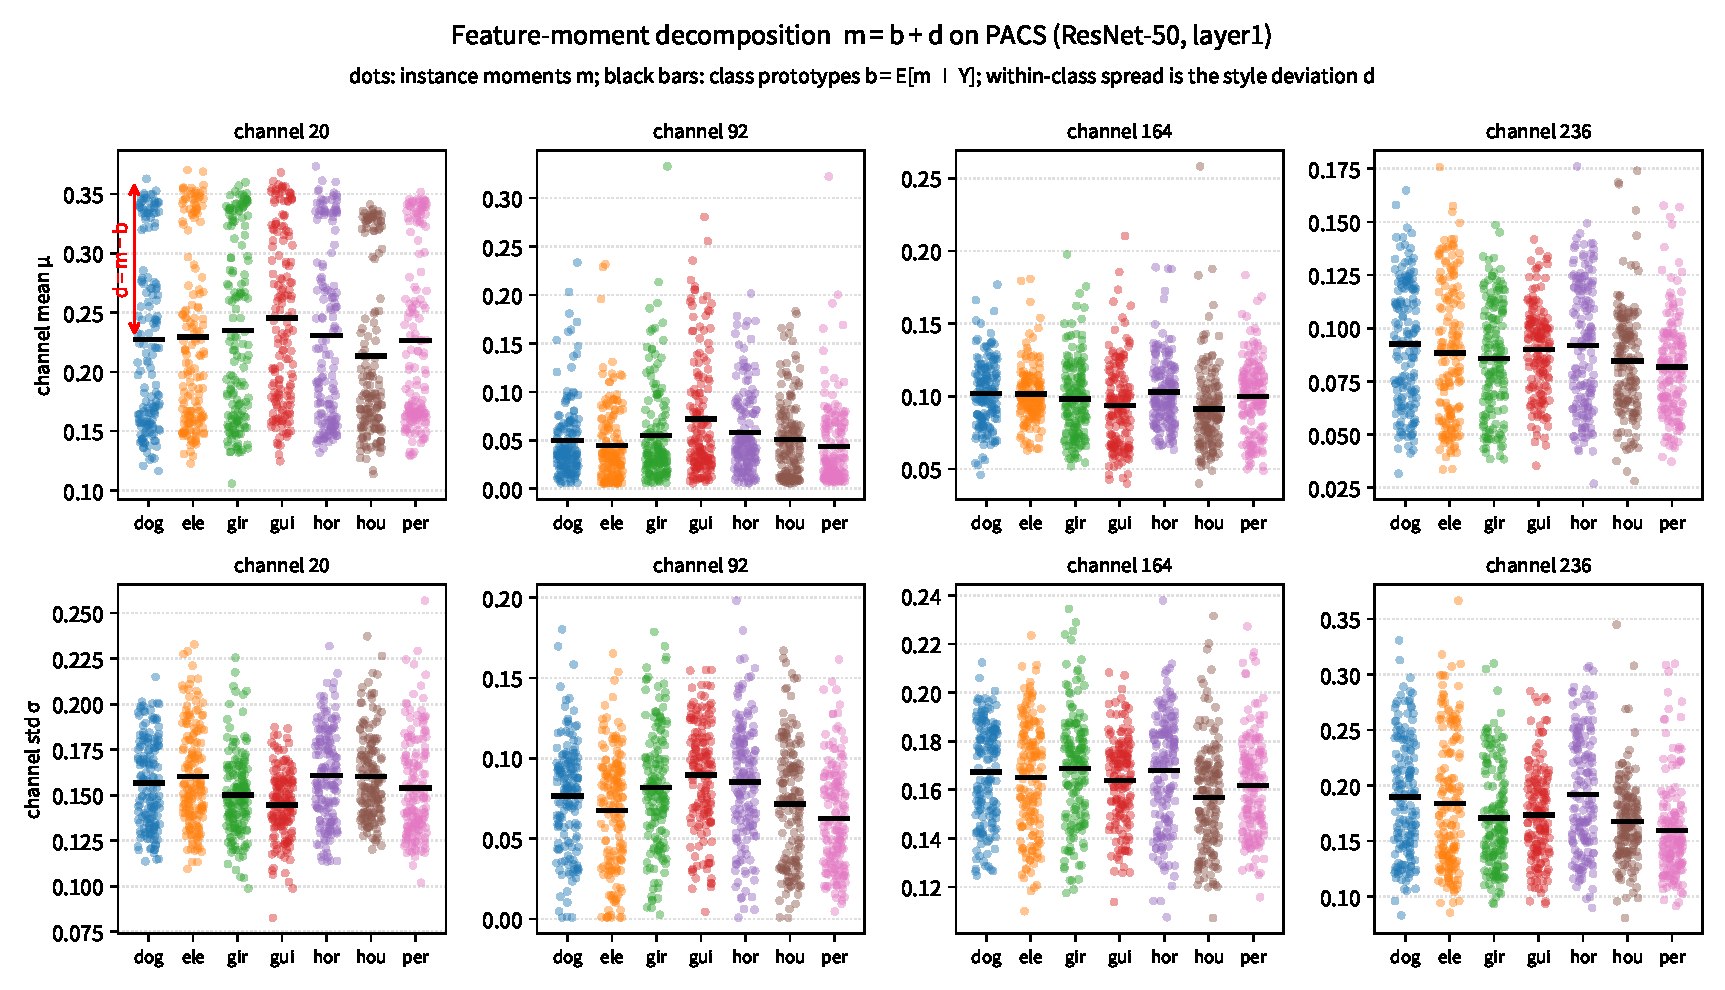
\includegraphics[width=\columnwidth]{fig_decomp.pdf}
\caption{Feature-moment decomposition on PACS (ResNet-50, layer1). For each selected channel, the dots are instance moments $\mathbf{m}$ over the four domains, colored by class, and the black bars are the class prototypes $\mathbf{b}=\mathbb{E}[\mathbf{m}\mid Y]$; the within-class spread is the style deviation $\mathbf{d}=\mathbf{m}-\mathbf{b}$. The statistics are computed on an ImageNet-pretrained backbone to illustrate the decomposition the operator uses.}
\label{fig:decomp}
\end{figure}

\noindent\textbf{Deviation mixing.} Given a partner instance $Z'$ with deviation $\mathbf{d}'$ and a coefficient $\lambda\in[0,1]$, form the mixed deviation
\begin{equation}
\mathbf{d}_{aug}=\lambda\,\mathbf{d}+(1-\lambda)\,\mathbf{d}'
\end{equation}
Equivalently, $\mathbf{d}_{aug}$ may be sampled from the empirical distribution of deviations (e.g., a fitted Gaussian), following the domain-randomization-uncertainty strategy. The augmented moments keep the baseline fixed and replace only the deviation:
\begin{equation}
\widetilde{\mu}_c=b_c^\mu+d_{aug,c}^\mu,\qquad
\widetilde{\sigma}_c=b_c^\sigma+d_{aug,c}^\sigma
\end{equation}
\begin{equation}
T(Z)=\widetilde{\sigma}\odot\frac{Z-\mu}{\sigma}+\widetilde{\mu}
\end{equation}
The operator is applied at layers $\mathcal{L}$ and triggered with probability $p$. To guard against violations of Assumption~2, we measure a \textbf{content-consistency} quantity
\begin{equation}
\mathrm{cons}(T;Z)=D\!\left(p(Y\mid Z)\,\Vert\,p(Y\mid T(Z))\right)
\end{equation}
where $D$ measures the divergence between the predicted (or class-prototype) distributions before and after augmentation; the view is accepted or down-weighted whenever $\mathrm{cons}\leq\delta$. By construction the baseline and normalized residual are never altered; augmentation resamples only the deviation.

\subsection{Feature-Space Content-Preserving Transformation}

We distinguish three levels: (L1) a strict style intervention in the generative model; (L2) the conditional feature-space statement the operator actually satisfies; and (L3) its empirical status in a trained network.

\noindent\textit{(L1) Strict style intervention in the generative model.} A transformation $T\in\mathcal{T}$ is a causal invariant transformation~\citep{ref22} when it preserves the causal feature, $g(T(X))=g(X)$. In the structural model of Assumption~1, consider the hard intervention $\mathrm{do}(S\!:=\!S')$ with an exogenous value $S'$ drawn independently, $S'\perp C$. It produces the counterfactual input
\begin{equation}
X_{S'}=g_0(C,S')
\end{equation}
Because $C$ is not a descendant of $S$ and $C\perp S$, the intervention changes neither the structural equation for $C$ nor its realized value, and the causal content of $X_{S'}$ equals that of $X$:
\begin{equation}
g(X_{S'})=C=g(X)
\end{equation}
Hence $\mathrm{do}(S\!:=\!S')$ is a CIT in the sense of~\citep{ref22}. This concerns the latent variables of the assumed model; the feature-moment operator instead acts on a learned $Z=\phi_l(X)$ through its channel statistics, and equating the two requires the feature-level condition next.

\noindent\textit{(Feature-level structural condition).} At a selected layer write $Z=\sigma(Z)\odot r(Z)+\mu(Z)$ with normalized residual $r(Z)=(Z-\mu(Z))/\sigma(Z)$. We posit the moment factorization
\begin{equation}
\mathbf{m}(Z)=\mathbf{b}(C)+\mathbf{d}(S)
\end{equation}
i.e., the baseline is determined by content and the deviation by style, together with \textbf{(feature sufficiency)} that the pair $(\mathbf{b}(Z),r(Z))$ is sufficient for content:
\begin{equation}
p\!\left(C\mid \mathbf{b}(Z),r(Z),\mathbf{d}(Z)\right)=p\!\left(C\mid \mathbf{b}(Z),r(Z)\right)
\end{equation}
This is the feature-space counterpart of $C\perp S$: once the content-bearing statistics are fixed, the deviation carries no further information about $C$.

\noindent\textbf{Proposition~1 (Conditional content preservation).} Under Assumptions~1--2 and the feature-level structural condition, with the mixing coefficient drawn independently of $C$:
\begin{itemize}[leftmargin=2.7em,labelwidth=2.3em,labelsep=0.4em,align=left]
\item[(L2-i)] in the idealized regime $\tau=0$ (so $\mathbf{d}\perp C$ and the partner source is exogenous), the operator preserves the content posterior exactly,
\begin{equation}
p(C\mid T(Z))=p(C\mid Z)
\end{equation}
\item[(L2-ii)] in the approximate regime, let the residual style--content dependence be bounded by $\tau$ in total variation, let the augmentation-family likelihood ratios satisfy $p(Z\mid C)/p(Z\mid C')\in[M^{-1},M]$, and write $p_{\min}=\min_c p(C)$. The primary bound is in total variation,
\begin{equation}
\mathrm{TV}\!\left(p(C\mid Z),\,p(C\mid T(Z))\right)\le \tau,
\label{eq:tvbound}
\end{equation}
which is exact under the coupling construction. As a valid corollary, under the uniform posterior lower bound $p(c\mid Z),p(c\mid T(Z))\ge q_{\min}=p_{\min}/M$, the KL divergence satisfies
\begin{equation}
D_{\mathrm{KL}}\!\left(p(C\mid Z)\,\Vert\,p(C\mid T(Z))\right)\le \frac{\tau}{q_{\min}}=\frac{\tau M}{p_{\min}}=:\varepsilon_C(\tau),
\label{eq:klcorollary}
\end{equation}
using the reverse-Pinsker-type inequality $D_{\mathrm{KL}}(P\Vert Q)\le \mathrm{TV}(P,Q)/q_{\min}$ (proved below); note that this replaces the earlier $\tau\log(M/p_{\min})$ bound, which is not valid in general. For the label posterior, when the divergence $D$ of Assumption~2(iii) is total variation, the triangle inequality gives
\begin{equation}
\mathrm{TV}\!\left(p(Y\mid Z),\,p(Y\mid T(Z))\right)\le \tau+\delta=:\varepsilon(\delta,\tau),
\label{eq:labeltv}
\end{equation}
so that both bounds vanish as $\tau,\delta\to0$. A KL label-posterior bound follows from \eqref{eq:klcorollary} applied to the label simplex under an analogous minimum-mass condition, but is not needed for the risk decomposition in Theorem~1, which is stated in total variation. The implemented content-consistency diagnostic (Eq.~(5)) uses KL between predictive distributions and should be read as an empirical monitor of prediction stability, not as a direct measurement of the latent content-posterior bound \eqref{eq:tvbound}.
\end{itemize}

\noindent\textit{Proof.}
\emph{Operator algebra.} By the defining equations of Section~\ref{sec:momentaug}, $T$ leaves $\mathbf{b}(Z)$ and $r(Z)$ unchanged and replaces only $\mathbf{d}(Z)$ by $\mathbf{d}_{aug}$.

\emph{Exact case (L2-i).} The replacement is the convex combination $\mathbf{d}_{aug}=\lambda\mathbf{d}+(1-\lambda)\mathbf{d}'$, with $\lambda$ independent of $C$. In the idealized regime $\mathbf{d}\perp C$ (Assumption~2(ii)) and $\mathbf{d}'\perp C$ (Assumption~2(iv)); a mixture of variables independent of $C$, with a content-independent coefficient, is itself independent of $C$, hence $\mathbf{d}_{aug}\perp C$. Under $\mathbf{m}(Z)=\mathbf{b}(C)+\mathbf{d}(S)$, replacing $\mathbf{d}(S)$ by an exogenous $\mathbf{d}_{aug}$ while holding $\mathbf{b}(C)$ and $r$ fixed is precisely the feature-space intervention $\mathrm{do}(S\!:=\!S_{aug})$: the content-determined statistics are untouched and only the style argument is exchanged for an exogenous value. Feature sufficiency then gives
\begin{equation*}
\begin{aligned}
p(C\mid T(Z))&=p\!\left(C\mid \mathbf{b}(Z),r(Z),\mathbf{d}_{aug}\right)\\
&=p\!\left(C\mid \mathbf{b}(Z),r(Z)\right)=p(C\mid Z)
\end{aligned}
\end{equation*}
where the middle equality uses that $(\mathbf{b},r)$ is sufficient and $\mathbf{d}_{aug}\perp C$. This proves (L2-i).

\emph{Approximate case (L2-ii).} Let $\mathbf{d}^{\perp}$ be the style-only correction of $\mathbf{d}$, i.e., the exogenous deviation with the same marginal but independent of $C$, and couple $(\mathbf{d},\mathbf{d}^{\perp})$ so that, conditionally and uniformly over $C$, $\mathrm{TV}(P_{\mathbf{d}\mid C},P_{\mathbf{d}^{\perp}\mid C})\le\tau$; this is precisely the residual dependence left after the class-conditional centering of Assumption~2(ii). Couple $\mathbf{d}_{aug}$ in the same way. Since the posterior $q(c)=p(c\mid \mathbf{b},r,\mathbf{d})$ is a measurable function of the observed statistics, the data-processing inequality for total variation transports the coupling discrepancy to the posterior without amplification:
\begin{equation}
\mathrm{TV}\!\left(p(C\mid Z),p(C\mid T(Z))\right)\le\tau,
\end{equation}
which is Eq.~\eqref{eq:tvbound}.

\emph{Valid KL corollary.} We prove the reverse-Pinsker-type bound
\begin{equation*}
D_{\mathrm{KL}}(P\Vert Q)\le \mathrm{TV}(P,Q)/q_{\min}
\end{equation*}
for any distributions $P,Q$ on a finite alphabet with $Q(c)\ge q_{\min}$. Let $A=\{c:P(c)\ge Q(c)\}$. On $A^c$ the contribution to $D_{\mathrm{KL}}$ is non-positive, so
\begin{equation*}
D_{\mathrm{KL}}(P\Vert Q)\le\sum_{c\in A}P(c)\log\frac{P(c)}{Q(c)}.
\end{equation*}
Using $\log x\le x-1$ for $x\ge1$,
\begin{equation*}
\sum_{A}P\log\frac{P}{Q}\le\sum_{A}P\Bigl(\frac{P}{Q}-1\Bigr)=\sum_{A}\frac{P(P-Q)}{Q}.
\end{equation*}
Writing $P=Q+(P-Q)$, the summand is $(P-Q)+(P-Q)^2/Q$, and on $A$ we have $P/Q\le 1/q_{\min}$, hence $(P-Q)^2/Q=(P-Q)(P/Q-1)\le(P-Q)(1/q_{\min}-1)$. Summing over $A$ and using $\sum_A(P-Q)=\mathrm{TV}(P,Q)$ gives
\begin{equation}
D_{\mathrm{KL}}(P\Vert Q)\le\mathrm{TV}(P,Q)+\Bigl(\frac{1}{q_{\min}}-1\Bigr)\mathrm{TV}(P,Q)=\frac{\mathrm{TV}(P,Q)}{q_{\min}}.
\label{eq:revpinsker}
\end{equation}
Bayes' rule under the likelihood-ratio condition gives, for every content value,
\begin{equation}
q(c)=\frac{p(Z\mid c)p(c)}{\sum_{c'}p(Z\mid c')p(c')}\ge \frac{p(c)}{M}\ge \frac{p_{\min}}{M}=:q_{\min},
\end{equation}
because $p(Z\mid c')\le M\,p(Z\mid c)$ and $\sum_{c'}p(c')=1$; the same bound holds for the post-augmentation posterior since $M$ bounds the likelihood ratios over the whole augmentation family. Applying \eqref{eq:revpinsker} with $\mathrm{TV}\le\tau$ yields Eq.~\eqref{eq:klcorollary}.

\emph{Label posterior.} The above bound concerns the content posterior, while classification ultimately cares about the label posterior. Since $Y=m(C,\xi)$ with $\xi\perp\!\!\!\perp C$, the label is content superimposed with independent noise; by the data-processing inequality for total variation, the portion of content-posterior drift transmitted to the label posterior is at most $\tau$. On the other hand, in Assumption~2(iii), the residual label-posterior change caused by replacing the style deviation does not exceed $\delta$ (when $D$ is total variation). The triangle inequality for total variation then gives
\begin{equation}
\mathrm{TV}\!\left(p(Y\mid Z),p(Y\mid T(Z))\right)\le\tau+\delta=\varepsilon(\delta,\tau),
\end{equation}
which is Eq.~\eqref{eq:labeltv}. Both bounds vanish as $\tau,\delta\to0$. A KL label-posterior bound can be obtained by applying \eqref{eq:revpinsker} to the label simplex under an analogous minimum-mass condition, but the primary statement and the subsequent risk decomposition (Theorem~1) use total variation, for which composition is exact. \hfill$\square$

\noindent\textit{(L3) Empirical status in a trained network.} In a deep network, the above idealizations do not hold exactly: a finite set of channel moments is not a sufficient statistic of $S$; the learned feature moments are not the latent style variable of Assumption~1; and the normalized residual and class prototype respectively retain some style information and instance-specific content (a class prototype is a class-conditional moment, not the causal content of an individual sample). Feature sufficiency therefore holds only approximately, and the resulting approximation error is absorbed by $\tau$ and monitored by the content-consistency measure $\mathrm{cons}$. We accordingly call $T$ an \emph{approximate feature-space content-preserving transformation under the recombination assumptions}, rather than a strict CIT; content preservation cannot be guaranteed by operator algebra alone, and the exogenous-source condition~2(iv) and (approximate) feature sufficiency are two indispensable, independently testable premises.

\subsection{Augmentation Family, Convex Ambiguity Set, and Generalization Bound}

Let the augmentation family $\mathcal{A}\subseteq\mathcal{T}$ induce the distribution family
\begin{equation}
\mathcal{P}_{\mathcal{A}}=\big\{P_T:T\in\mathcal{A}\big\}
\end{equation}
The ambiguity set is taken to be the closed convex hull of this family (rather than a linear span of directions),
\begin{equation}
\mathcal{U}_{\mathcal{A}}=\overline{\operatorname{conv}}\big(\mathcal{P}_{\mathcal{A}}\big)
\end{equation}
i.e., all mixtures of augmented distributions. The corresponding robust objective is
\begin{equation}
\min_h\ \sup_{Q\in\mathcal{U}_{\mathcal{A}}}R_Q(h)
\end{equation}
This convex-hull minimax is the distribution-space analogue of the risk-extrapolation (REx) idea~\citep{ref43}: REx constructs its uncertainty set through affine extrapolation of training risks, whereas here the hull is built explicitly from feature-moment-induced distributions, so the coverage gap can be expressed through the style deviation and monitored empirically. Total variation adopts the coupling convention,
\begin{equation}
\mathrm{TV}(P,Q)=\frac{1}{2}\int\left|dP-dQ\right|
\end{equation}
under which the risk inequality below has constant one.

\noindent\textbf{Admissible shift space and convex-hull coverage.} Let $\mathcal{S}_{\mathrm{adm}}$ denote the set of admissible style marginals for the target domain. A target distribution $P_{te}$ has style variable $S_{te}\in\mathcal{S}_{\mathrm{adm}}$ and, by Assumption~1, the target domain shares the content mechanism and content distribution with the source domains. The convex hull $\mathcal{U}_{\mathcal{A}}$ \emph{exactly covers} the admissible shift space if
\begin{equation}
\{P_{te}:S_{te}\in\mathcal{S}_{\mathrm{adm}}\}\subseteq\mathcal{U}_{\mathcal{A}}
\end{equation}
and an \emph{$\eta$-approximate coverage} if
\begin{equation}
\sup_{S_{te}\in\mathcal{S}_{\mathrm{adm}}} d_{\mathrm{TV}}(P_{te},\mathcal{U}_{\mathcal{A}})\ \le\ \eta
\end{equation}
We call $\eta$ the \emph{coverage gap}.

\noindent\textbf{Theorem~1 (Conditional OOD generalization bound).} Let the loss be bounded, $\ell\in[0,\ell_{\max}]$, and define the target-to-ambiguity distance by
\begin{equation}
d_{\mathrm{TV}}(P_{te},\mathcal{U}_{\mathcal{A}})=\inf_{Q\in\mathcal{U}_{\mathcal{A}}}\mathrm{TV}(P_{te},Q)
\end{equation}
Then, for every predictor $h$:
(i) if $P_{te}\in\mathcal{U}_{\mathcal{A}}$, $R_{P_{te}}(h)\leq\sup_{Q\in\mathcal{U}_{\mathcal{A}}}R_Q(h)$;
(ii) in general,
\begin{equation}
R_{P_{te}}(h)\ \leq\ \sup_{Q\in\mathcal{U}_{\mathcal{A}}}R_Q(h)\;+\;\ell_{\max}\,d_{\mathrm{TV}}(P_{te},\mathcal{U}_{\mathcal{A}})
\end{equation}
and (iii) \emph{(coverage characterization)} the gap vanishes if and only if $P_{te}\in\overline{\mathrm{conv}}(\mathcal{P}_{\mathcal{A}})$, i.e., \del{if and only if \mbox{$P_{te}$} is a convex combination of distributions in \mbox{$\mathcal{P}_{\mathcal{A}}$}, which by Carath\'eodory's theorem uses at most \mbox{$d+1$} terms in an affine hull of dimension \mbox{$d$}, where the affine-hull dimension \mbox{$d$} is finite because every \mbox{$P_T$} is indexed by the finite-dimensional channel-moment vector at the selected layers;}\add{if and only if $P_{te}$ admits a convex-combination representation by distributions in $\mathcal{P}_{\mathcal{A}}$ (this is the defining property of the closed convex hull, not a consequence of finite-dimensional parameterization). For the finite empirical hull with $s$ realized operators, any such representation uses at most $s$ terms. We do not assert a universal $d+1$ reduction in the ambient measure space: finite-dimensional parameterization of the channel moments does not by itself imply a finite-dimensional affine hull of the induced distribution family, because the map from moments to distributions is nonlinear;} this conclusion is independent of whether the admissible shift space is finite or continuous, since finiteness of the shift space alone does not imply containment. If the hull is an $\eta$-approximate coverage, then $d_{\mathrm{TV}}(P_{te},\mathcal{U}_{\mathcal{A}})\leq\eta$ and the corresponding risk additive term is at most $\ell_{\max}\eta$. For the finite empirical hull $\mathcal{U}_{\mathcal{A}}^{(s)}=\mathrm{conv}\{P_{T_1},\ldots,P_{T_s}\}\subseteq\mathcal{U}_{\mathcal{A}}$, writing $h_s=\sup_{Q\in\mathcal{U}_{\mathcal{A}}}d_{\mathrm{TV}}(Q,\mathcal{U}_{\mathcal{A}}^{(s)})$,
\begin{equation}
d_{\mathrm{TV}}(P_{te},\mathcal{U}_{\mathcal{A}}^{(s)})\ \leq\ \eta+h_s
\end{equation}
where $h_s$ \del{depends only on the training distribution and can be directly computed at training time}\add{depends only on training-side distributions and is estimated empirically at training time---by sampling additional augmentations and measuring their TV distance to the empirical hull on the source holdout} (with $h_s\to0$ as the empirical operators become dense in $\mathcal{P}_{\mathcal{A}}$), whereas $\eta=d_{\mathrm{TV}}(P_{te},\mathcal{U}_{\mathcal{A}})$ is target-dependent and is not identifiable without target access.

\noindent\textit{Proof.}
\emph{(i)} Write $P_{te}=\sum_k\alpha_k P_{T_k}$ with $\alpha_k\geq0$, $\sum_k\alpha_k=1$ (the closed-hull case follows by taking limits). Since risk is affine in the distribution,
\begin{equation}
R_{P_{te}}(h)=\sum_k\alpha_k R_{P_{T_k}}(h)\leq\max_k R_{P_{T_k}}(h)\leq\sup_{Q\in\mathcal{U}_{\mathcal{A}}}R_Q(h)
\end{equation}

\emph{(ii)} Let $Q^*\in\mathcal{U}_{\mathcal{A}}$ attain (or $\varepsilon$-attain) the infimum. For $\ell\in[0,\ell_{\max}]$, take an optimal coupling such that $P(X\neq X')=\mathrm{TV}(P,Q)$; the loss difference is zero on the matching set and bounded by $\ell_{\max}$ on the disagreement set, yielding the total-variation risk inequality
\begin{equation}
|R_P(h)-R_Q(h)|\leq\ell_{\max}\,\mathrm{TV}(P,Q)
\end{equation}
with constant one under the coupling convention above. Then
\begin{equation*}
\begin{aligned}
R_{P_{te}}(h)&\leq R_{Q^*}(h)+|R_{P_{te}}(h)-R_{Q^*}(h)|\\
&\leq\sup_{Q\in\mathcal{U}_{\mathcal{A}}}R_Q(h)+\ell_{\max}\,\mathrm{TV}(P_{te},Q^*)
\end{aligned}
\end{equation*}
and taking the infimum over $Q^*$ yields (ii).

\emph{(iii)} Since $\mathcal{U}_{\mathcal{A}}$ is closed and convex, $d_{\mathrm{TV}}(P_{te},\mathcal{U}_{\mathcal{A}})=0$ if and only if $P_{te}\in\mathcal{U}_{\mathcal{A}}=\overline{\mathrm{conv}}(\mathcal{P}_{\mathcal{A}})$, which is exactly the convex-combination representation\add{ by definition}. \del{Carath\'eodory's theorem in the affine hull of \mbox{$\mathcal{P}_{\mathcal{A}}$} (dimension at most \mbox{$d$}) reduces any such combination to at most \mbox{$d+1$} members, all belonging to \mbox{$\mathcal{P}_{\mathcal{A}}$} whether the shift space \mbox{$\mathcal{S}_{\mathrm{adm}}$} is discrete or continuous.}\add{For the finite empirical hull with $s$ members, any representation uses at most $s$ terms. We do not invoke a universal $d+1$ reduction: in the ambient measure space, finite-dimensional channel-moment parameterization does not imply a finite-dimensional affine hull of the induced distributions because the moment-to-distribution map is nonlinear.} Note, however, that finiteness of $\mathcal{S}_{\mathrm{adm}}$ alone does not guarantee that $P_{te}$ lies in the hull of the realized operators. The $\eta$-approximate coverage condition is $\sup_{S_{te}}d_{\mathrm{TV}}\leq\eta$ by definition, which substituted into (ii) gives an upper bound of $\ell_{\max}\eta$ on the additive term.

For the finite hull, choose $Q^*\in\mathcal{U}_{\mathcal{A}}$ with $\mathrm{TV}(P_{te},Q^*)\leq\eta+\varepsilon$, and then $Q_s\in\mathcal{U}_{\mathcal{A}}^{(s)}$ with $\mathrm{TV}(Q^*,Q_s)\leq h_s+\varepsilon$, which is guaranteed by the definition of $h_s$. The triangle inequality gives
\begin{equation}
d_{\mathrm{TV}}(P_{te},\mathcal{U}_{\mathcal{A}}^{(s)})\leq\mathrm{TV}(P_{te},Q_s)\leq\eta+h_s+2\varepsilon
\end{equation}
Since this holds for every $\varepsilon>0$, letting $\varepsilon\to0$ yields $d_{\mathrm{TV}}(P_{te},\mathcal{U}_{\mathcal{A}}^{(s)})\leq\eta+h_s$. \del{Since \mbox{$h_s$} depends only on training-side distributions, when the empirical operators become dense in \mbox{$\mathcal{P}_{\mathcal{A}}$},}\add{Since $h_s$ depends only on training-side distributions, it is estimated by sampling additional augmentations and measuring their TV distance to the empirical hull. As the empirical operators become dense in $\mathcal{P}_{\mathcal{A}}$,} the finite hull $\mathcal{U}_{\mathcal{A}}^{(s)}$ increases monotonically to the full hull $\mathcal{U}_{\mathcal{A}}$, and hence $h_s\to0$. The residual $\eta$ depends on the target domain $P_{te}$, so without target access it can neither be computed nor bounded from above by training data. \hfill$\square$

\noindent\textit{Remark (scope of the error bound).} Part~(ii) is the standard, unconditional total-variation risk decomposition; part~(iii) only makes the uncovered portion explicit and does not provide a target-free guarantee. Training-side statistics (namely, the coverage width of augmented distributions on the source holdout and the support of the empirical deviation distribution) \del{monitor \mbox{$h_s$} and the family's reach, but}\add{provide empirical estimates of $h_s$ and the family's reach---sample additional augmentations and measure their TV distance to the empirical hull; these are estimates, not exact computations. None} can give an upper bound on $\eta$ without an added assumption relating deployment style to the sources. The error bound is conditional on coverage, which is partly untestable at training time. The same holds with $\chi^2$ or other $f$-divergences, with constants adjusted accordingly.

Fig.~\ref{fig:coverage} illustrates the two terms in a controlled moment-space setting: the target-dependent gap $\eta$ and the source-side term $h_s$.

\begin{figure}[t]
\centering
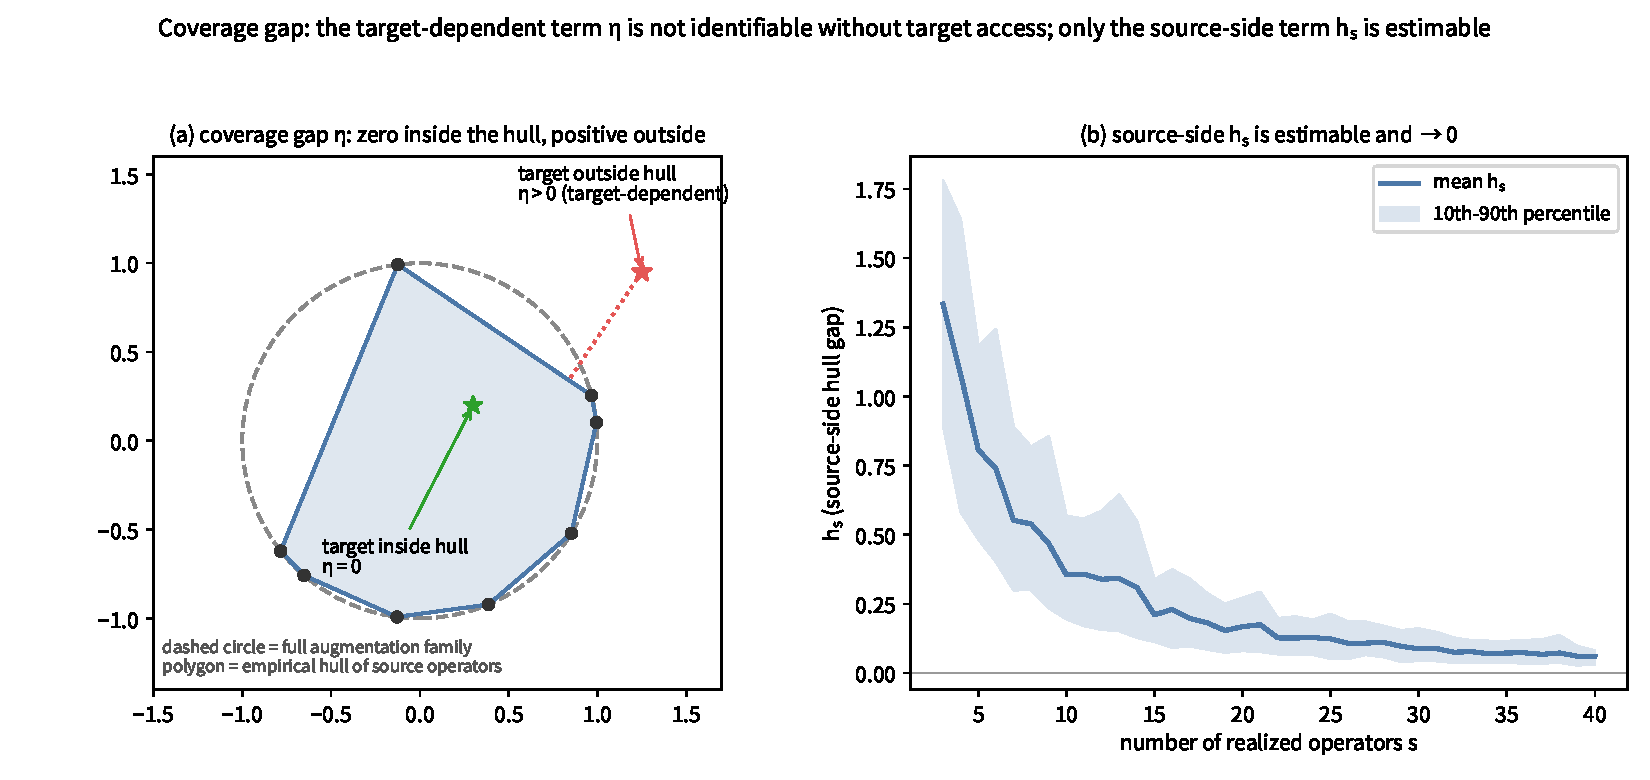
\includegraphics[width=\columnwidth]{fig_coverage.pdf}
\caption{Coverage-gap terms in Theorem 1 (synthetic illustration in moment space). (a) The target-dependent gap $\eta$ is zero when the target lies in the convex hull of the source augmentation family and positive otherwise. (b) The source-side term $h_s$ is the distance from the full augmentation family to the empirical hull; it is estimable on the source holdout and tends to zero as the number of realized operators grows. The real target-dependent gap $\eta$ cannot be computed or bounded without target access, so this figure illustrates the mechanism only.}
\label{fig:coverage}
\end{figure}

\noindent\textbf{Proposition~2 (Tightest bound and cost of robustness).} Let $h_R=\arg\min_h\sup_{Q\in\mathcal{U}_{\mathcal{A}}}R_Q(h)$, assume the unaugmented training distribution is retained, $P_{tr}\in\mathcal{U}_{\mathcal{A}}$, and define the hull radius
\begin{equation}
\operatorname{rad}(\mathcal{U}_{\mathcal{A}})=\sup_{Q\in\mathcal{U}_{\mathcal{A}}}\mathrm{TV}(Q,P_{tr})
\end{equation}
Then, for every predictor $h$,
\begin{equation}
R_{P_{te}}(h_R)\ \leq\ \sup_{Q\in\mathcal{U}_{\mathcal{A}}}R_Q(h)\;+\;\ell_{\max}\,d_{\mathrm{TV}}(P_{te},\mathcal{U}_{\mathcal{A}})
\end{equation}
i.e., the robust solution attains the tightest bound of Theorem~1. Meanwhile, the risk increase of ERM ($h_E=\arg\min_h R_{P_{tr}}(h)$) within the augmentation family is bounded by
\begin{equation}
\sup_{Q\in\mathcal{U}_{\mathcal{A}}}R_Q(h_E)-R_{P_{tr}}(h_E)\ \leq\ \ell_{\max}\operatorname{rad}(\mathcal{U}_{\mathcal{A}})
\end{equation}
Note that the above assumptions do not guarantee $R_{P_{te}}(h_R)\leq R_{P_{te}}(h_E)$, since the robust optimum attaining the tightest bound only provides conditions for target-domain improvement and does not imply that the actual target risk is necessarily lower.

\noindent\textit{Proof.} We prove in three steps: first the tightest bound, then the cost-of-robustness bound, and finally a supplementary observation.

\emph{(Tightest bound).} We first show that $h_R$ attains the tightest bound. Applying Theorem~1(ii) to $h_R$,
\begin{equation}
R_{P_{te}}(h_R)\ \leq\ \sup_{Q\in\mathcal{U}_{\mathcal{A}}}R_Q(h_R)+\ell_{\max}d_{\mathrm{TV}}(P_{te},\mathcal{U}_{\mathcal{A}}).
\end{equation}
Because $h_R$ attains the minimum worst-case risk, $\sup_Q R_Q(h_R)\leq\sup_Q R_Q(h)$ for every predictor $h$; substituting yields the tightest bound for $h_R$ under Theorem~1, since every predictor's part-(ii) bound is composed of the same two terms and $h_R$ minimizes the worst-risk term $\sup_Q R_Q(h)$, hence its upper bound is the smallest.

\emph{(Cost-of-robustness bound).} For any $Q\in\mathcal{U}_{\mathcal{A}}$, combining the total-variation risk inequality under the coupling convention (constant one), the definition of the radius, and $P_{tr}\in\mathcal{U}_{\mathcal{A}}$, we obtain
\begin{equation}
\begin{aligned}
R_Q(h_E)-R_{P_{tr}}(h_E)&\leq |R_Q(h_E)-R_{P_{tr}}(h_E)|\\
&\leq \ell_{\max}\mathrm{TV}(Q,P_{tr})\leq \ell_{\max}\operatorname{rad}(\mathcal{U}_{\mathcal{A}}).
\end{aligned}
\end{equation}
Taking the supremum over $Q\in\mathcal{U}_{\mathcal{A}}$ yields the worst-case risk loss bound of ERM within the augmentation family.

\emph{(Supplementary observation).} The Theorem~1(ii) bounds of both $h_R$ and $h_E$ contain the same additive term $\ell_{\max}d_{\mathrm{TV}}(P_{te},\mathcal{U}_{\mathcal{A}})$. Since this additive term is independent of the choice of predictor, nothing in the assumptions allows comparison of their actual target risks. \hfill$\square$

\subsection{Weight Averaging and Trajectory Ensemble}

Let $\{h_t\}$ be densely saved checkpoints from late training, with parameters $\theta_t$ (i.e., $h_t(x)=h(x;\theta_t)$), and weights $w_t\geq 0$, $\sum_t w_t=1$. We distinguish two aggregation schemes: the \textbf{weight-averaged network}
\begin{equation}
\bar h(x)=h(x;\bar\theta),\qquad \bar\theta=\sum_t w_t\theta_t
\end{equation}
and the \textbf{trajectory ensemble}
\begin{equation}
h_{ens}(x)=\sum_t w_t h(x;\theta_t).
\end{equation}
Since for predictors linear in the parameters we have $h(x;\sum_t w_t\theta_t)=\sum_t w_t h(x;\theta_t)$, the two coincide (for nonlinear networks this equality generally fails, so they are not equivalent). Writing $\Delta_t=\theta_t-\bar\theta$, we have $\sum_t w_t\Delta_t=0$ because $\sum_t w_t=1$.

\noindent\textbf{Assumption~3 (Trajectory--augmentation alignment).} Within the flat parameter neighborhood selected by the dense averaging window, the empirical distribution of trajectory checkpoints $\{\theta_t\}$ approximates the distribution of predictors induced by the augmentation family. This idea comes from the local-Bayesian weight-space view behind SWA and SWAD~\citep{ref42}: densely sampled late-trajectory weights can therefore be viewed as samples from the predictor distribution induced by augmented views. This is also consistent with the observation of Zhou et al.~\citep{ref4} that weight averaging is orthogonal to the direction of domain shift, and is therefore commonly used as a post-processing method for domain generalization.

\add{We treat Assumption~3 as an empirically supported assumption rather than a proven theorem, and verify it next.}

\add{\noindent\textbf{Empirical verification.} We test Assumption~3 on two PACS target domains (sketch and art\_painting), with four independent seeds per domain (16 runs in total), comparing SWAD-window checkpoints against ERM checkpoints in both prediction and feature spaces. In the prediction space, the nearest-neighbor ratio (one being perfect) of SWAD checkpoints to the CIFA augmentation family is 1.23 versus 2.14 for ERM, and the mean prediction KL is 0.036 versus 0.072 nats; both hold for 8/8 runs (paired $p=0.000005$ and $p=0.0004$). In the feature space, the nearest-neighbor distance of SWAD checkpoints to augmented features is only 39\% (layer1) and 47\% (layer2) of the ERM distance (8/8, $p<10^{-6}$, paired Cohen's $d\approx-8.7$), the feature-moment KL is 0.29 and 0.33 of the ERM value (Wilcoxon $p=0.008$), and CKA agrees in direction with a small absolute difference (1--3\%). These two independent lines of evidence consistently support the alignment of the trajectory with the augmentation family.}

\add{The verification has four limitations: it covers only two PACS domains; the SWAD window is short; the dispersion of augmentations (0.017) is much smaller than that of the trajectory checkpoints (0.155), so the correct reading is that the augmentation family is \emph{covered by} rather than distributionally identical to the trajectory; and the result is not a causal proof. We therefore present Assumption~3 as an empirically supported assumption rather than a proven theorem.}

\noindent\textbf{Theorem~2 (Weight averaging approximates the trajectory ensemble).} Let the prediction space $\mathcal{H}$ be endowed with norm $\|\cdot\|_{\mathcal{H}}$ (the probability simplex for classification, $\mathbb{R}$ for regression), and the parameter space take the Euclidean norm $\|\cdot\|_2$. Assume:
(a) convex loss: for every $y$, $\ell(\cdot,y):\mathcal{H}\to\mathbb{R}$ is convex;
(b) Lipschitz loss: $\ell$ is $L_{\ell}$-Lipschitz under $\|\cdot\|_{\mathcal{H}}$;
(c) local second-order regularity: on the line segment joining $\bar\theta$ to each $\theta_t$, \del{the Hessian of the predictor map \mbox{$\theta\mapsto h(x;\theta)$} satisfies the quadratic-form bound}\add{the predictor map $\theta\mapsto h(x;\theta)$ is twice continuously differentiable and its Hessian satisfies the quadratic-form bound}
\begin{equation}
\|\Delta^{\top}\nabla_{\theta}^{2}h(x;\theta)\Delta\|_{\mathcal{H}}\ \leq\ \kappa\,\|\Delta\|_{2}^{2}.
\end{equation}
\del{For networks containing ReLU or BatchNorm, this holds except at non-differentiable points (which have measure zero), with \mbox{$\kappa$} the essential supremum.}\add{For smooth activations (GELU, softplus, tanh) this is a strict statement. For ReLU or BatchNorm the map is only piecewise C$^2$ and a segment may cross activation boundaries, so the theorem is read as an approximation: the integral Taylor remainder (proof below) adds a kink term that is small in the flat SWAD window and is, together with $\kappa$, estimated from the checkpoints rather than assumed.}
Writing $\Delta_t=\theta_t-\bar\theta$ and $r=\max_t\|\Delta_t\|_2$:
(i) for every distribution $Q$,
\begin{equation}
R_Q(h_{ens})\leq\sum_t w_t R_Q(h_t)
\end{equation}
(ii) for every distribution $Q$,
\begin{equation}
\left|R_Q(\bar h)-R_Q(h_{ens})\right|\leq\frac{L_{\ell}\kappa}{2}\,r^{2}
\end{equation}
Theorem~2 only characterizes how well the weight-averaged network approximates its own trajectory ensemble; whether that ensemble can be viewed as augmentation-family predictors depends on Assumption~3.

\noindent\textit{Proof.}
\emph{(i)} Fix $(x,y)$. By definition $h_{ens}(x)=\sum_t w_t h(x;\theta_t)$ with $\sum_t w_t=1$. Convexity of $\ell(\cdot,y)$ and Jensen's inequality give
\begin{equation}
\ell(h_{ens}(x),y)=\ell\!\left(\sum_t w_t h_t(x),y\right)\leq\sum_t w_t\,\ell(h_t(x),y)
\end{equation}
Taking the expectation over $(x,y)\sim Q$ yields $R_Q(h_{ens})\leq\sum_t w_t R_Q(h_t)$.

\emph{(ii)} Fix $x$. \del{The second-order Taylor expansion of \mbox{$\theta\mapsto h(x;\theta)$} at \mbox{$\bar\theta$} along \mbox{$\Delta_t$} is}\add{Under (c), the second-order Taylor expansion at $\bar\theta$ along $\Delta_t$ is}
\begin{equation}
h(x;\theta_t)=\bar h(x)+\nabla_{\theta}h(x;\bar\theta)^{\top}\Delta_t+\frac{1}{2}\Delta_t^{\top}\nabla_{\theta}^{2}h(x;\zeta_t)\Delta_t
\end{equation}
\del{with \mbox{$\zeta_t$} on the segment between \mbox{$\bar\theta$} and \mbox{$\theta_t$} (under the almost-everywhere reading, apply on the differentiable set and bound by the essential supremum).}\add{For piecewise C$^2$ networks, write $\gamma_t(s)=\bar\theta+s\Delta_t$ and apply the integral form on each C$^2$ piece; crossing an activation boundary at $s_i$ adds the kink term $(1-s_i)[\nabla h(x;\gamma_t(s_i+))-\nabla h(x;\gamma_t(s_i-))]^{\top}\Delta_t$. The interior Hessian integral is bounded by $(\kappa/2)\|\Delta_t\|^2$; the kink term is not controlled by $\kappa$ and is estimated empirically. Under the strict C$^2$ reading there are no kinks and the displayed bound follows exactly; under the ReLU reading it is approximate with the residual kink monitored on the checkpoints.} Multiply by $w_t$ and sum over $t$. Because
\begin{equation}
\sum_t w_t\Delta_t=\sum_t w_t(\theta_t-\bar\theta)=\bar\theta-\bar\theta=0
\end{equation}
the first-order term cancels\add{ and, under the strict C$^2$ reading,}
\begin{equation}
h_{ens}(x)-\bar h(x)=\frac{1}{2}\sum_t w_t\,\Delta_t^{\top}\nabla_{\theta}^{2}h(x;\zeta_t)\Delta_t
\end{equation}
\add{so} Taking the prediction-space norm and using the quadratic-form bound with $\|\Delta_t\|_2\leq r$,
\begin{equation}
\|h_{ens}(x)-\bar h(x)\|_{\mathcal{H}}\leq\frac{1}{2}\sum_t w_t\,\kappa\|\Delta_t\|_2^{2}\leq\frac{\kappa}{2}r^{2}\add{+\varepsilon_{\mathrm{kink}}}
\end{equation}
\add{where under the piecewise-C$^2$ (ReLU) reading $\varepsilon_{\mathrm{kink}}$ is the empirical kink residual, measured directly as the portion of $\|h_{ens}-\bar h\|$ not explained by the interior Hessian term.} The Lipschitz condition on the loss then gives, for each $(x,y)$,
\begin{equation}
|\ell(\bar h,y)-\ell(h_{ens},y)|\leq L_{\ell}\|\bar h-h_{ens}\|_{\mathcal{H}}\leq\frac{L_{\ell}\kappa}{2}r^{2}\add{+L_{\ell}\varepsilon_{\mathrm{kink}}}
\end{equation}
Taking the expectation and using $|R_Q(\bar h)-R_Q(h_{ens})|\leq\mathbb{E}_Q|\ell(\bar h,y)-\ell(h_{ens},y)|$ yields (ii)\add{, exactly under the strict C$^2$ reading and up to the empirical kink residual under the ReLU reading}. \hfill$\square$

\textit{Remark (Worst-case excess-risk decomposition).} Combining part (ii) with the optimization and sampling structure decomposes the worst-case excess of the averaged predictor,
\begin{equation}
\sup_{Q\in\mathcal{U}_{\mathcal{A}}}R_Q(\bar h)-\inf_h\sup_{Q\in\mathcal{U}_{\mathcal{A}}}R_Q(h)\ \leq\ \frac{L_\ell\,\kappa}{2}r^{2}+\varepsilon_{\mathrm{avg}}
\end{equation}
where $\varepsilon_{\mathrm{avg}}=\varepsilon_{\mathrm{disc}}+\varepsilon_{\mathrm{opt}}+\varepsilon_{\mathrm{fs}}$ collects, respectively, the finite-checkpoint discretization gap of the trajectory ensemble, the optimization error at termination, and the finite-sample error of the empirical minimax problem. These terms are not bounded by the theorem and are treated as empirical quantities; standard orders are $O(T^{-1/2})$-type for discretization with $T$ checkpoints under mixing, and $O(\sqrt{\log|\mathcal{E}|/n})$-type for finite-sample group-minimax generalization~\citep{ref10}. Under Assumption~3 the same decomposition is read relative to the augmentation family; without it, the strict statement relates $\bar h$ only to its own trajectory ensemble.

\textit{Remark.} Because averaging is taken at the barycenter, the first-order term cancels and the leading error is \emph{quadratic} in the neighborhood radius; this is the precise sense in which dense averaging seeks a flat minimum. It directly controls the neighborhood aggregated risk, while worst-case risk is controlled only jointly with curvature and radius. We do not claim averaging alone solves the strict minimax problem.

\subsection{The CIFA Algorithm}
\label{sec:algorithm}

Algorithm~\ref{alg:cifa} summarizes the CIFA procedure. We formulate CIFA as a unified framework that combines feature-moment augmentation, content-consistency guards, soft worst-case aggregation, and dense weight averaging in a single objective \add{designed to be backbone-agnostic}:
\begin{equation}
\min_h\ \mathbb{E}_{(X,Y)\sim P_{tr}}\!\left[\ell\big(h(X),Y\big)+\lambda_c\,\mathrm{cons}\big(T;X\big)\right]
\end{equation}
where $T$ is applied at layers $\mathcal{L}$ with probability $p$. The original and augmented views are aggregated via soft worst-case weights, and the final output is the dense weight average $\bar h$. The soft worst-case weights over $K$ views are
\begin{equation}
q_k=\frac{\exp(\beta R_k)}{\sum_{j=1}^{K}\exp(\beta R_j)}
\end{equation}
which smoothly interpolates between uniform averaging ($\beta\to 0$) and worst-case averaging ($\beta\to\infty$). The gate and consistency term are protection mechanisms: under mild augmentations the gate stays at one and the consistency penalty is negligible, adding no measurable gain. They down-weight a view only when the augmentation moves the prediction beyond the tolerance $\delta$.

\noindent\textbf{Relation to the minimax objective.} CIFA training is a finite-sample soft relaxation of $\min_h\sup_{Q\in\mathcal{U}_{\mathcal{A}}}R_Q(h)$, differing from exact solution in three respects. First, at finite $\beta$ the soft aggregation is a $\log$-sum-exp approximation to the maximum over $K$ views,
\begin{equation}
0\ \leq\ \frac{1}{\beta}\log\sum_{k=1}^{K}e^{\beta R_k}-\max_k R_k\ \leq\ \frac{\log K}{\beta}
\end{equation}
and this difference vanishes only as $\beta\to\infty$. Second, only $K$ finite views are realized per step, an inner approximation of the full family that corresponds to the finite-sample term $\varepsilon_{\mathrm{fs}}$ and the hull-discretization term $h_s$ of Theorem~1. Third, the dense weight average is the parameter-space approximation of Theorem~2, requiring Assumption~3 to be identified with aggregation over augmented predictors. CIFA therefore approximates a finite-sample soft robust objective associated with $\mathcal{P}_{\mathcal{A}}$, rather than being an exact solver of the convex-hull minimax problem.

\begin{algfloat}
\caption{The CIFA algorithm.}
\label{alg:cifa}
\fontsize{7.6}{9.2}\ttfamily
\setlength{\tabcolsep}{3pt}
\begin{tabular}{p{0.97\columnwidth}}
\toprule
\rmfamily\textbf{Input}: source domains; layer set $\mathcal{L}$; trigger prob.\ $p$; mixing range $\lambda$; KL tolerance $\delta$; soft-worst coefficient $\beta$; baseline momentum; SWAD window schedule\\
\midrule
1\hspace{0.6em}for each training iteration do\\
2\hspace{1.2em}sample a minibatch from the source domains\\
3\hspace{1.2em}compute instance moments $(\mu,\sigma)$ at layers $\mathcal{L}$\\
4\hspace{1.2em}update content baseline $b$ (class-prototype EMA; global EMA fallback)\\
5\hspace{1.2em}for each layer $l$ in $\mathcal{L}$ do\\
6\hspace{1.8em}with trigger probability $p$:\\
7\hspace{2.4em}compute style deviation $d=m-b$\\
8\hspace{2.4em}draw a partner deviation $d'$ (a derangement over\\
9\hspace{3.0em}the whole minibatch, not restricted to the same class) and $\lambda$\\
10\hspace{2.4em}form $d_{aug}=\lambda d+(1-\lambda)d'$ (or sample from\\
11\hspace{3.0em}the batch's empirical deviation distribution)\\
12\hspace{2.4em}recompose $m_{aug}=b+d_{aug}$ and the view $T(Z)$\\
13\hspace{2.4em}compute $\mathrm{cons}=D_{\mathrm{KL}}(p_c\|p_a)$; set the gate\\
14\hspace{3.0em}$g=\min\{1,\delta/(\mathrm{cons}+10^{-8})\}$ (soft down-weight)\\
15\hspace{1.2em}compute losses on the original and augmented views\\
16\hspace{1.2em}aggregate views with soft worst-case weights $q_k=\mathrm{softmax}(\beta R_k)$; update $h$\\
17\hspace{1.2em}update the dense weight-averaging window (EMA of checkpoints)\\
18 end\\
\bottomrule
\rmfamily\textbf{Output}: weight-averaged predictor $\bar h$\\
\end{tabular}
\end{algfloat}

\add{\noindent\textbf{Baseline initialization, few-shot classes, and partner sampling.} The per-class prototype buffers are initialized to zero together with a per-class seen flag. On the first occurrence of a class, the prototype is set directly to that class's mean moments in the batch (rather than accumulating from zero); subsequent batches update it by an exponential moving average with momentum 0.9. A global EMA over all instances is maintained in parallel; instances of a class not yet observed, including few-shot classes early in training, fall back to this global baseline rather than to zero. The partner deviation is drawn by a derangement over the whole minibatch, so each instance is paired with another instance regardless of class---i.e., partners come from the batch's empirical deviation distribution, not from the same class only. An alternative Gaussian mode draws partners from the batch's empirical deviation distribution in the DSU style. No hard rejection is applied: the gate is the soft factor $g=\min\{1,\delta/(\mathrm{cons}+10^{-8})\}$, which equals one whenever the KL is below $\delta$ and smoothly down-weights the augmented view otherwise.}

\noindent\textbf{Gradient-flow (stop-gradient) details.} To ensure training stability under finite samples and prevent augmentation statistics from interfering with gradient backpropagation, three quantities enter the objective as constants with their gradients stopped, exactly as in the released code. (i)~The content baseline $b$ is a class-prototype exponential moving average updated from detached clean moments, so no gradient flows back through the prototype. (ii)~The moments $(\mu,\sigma)$, the mixed deviation, the partner deviation, and the mixing coefficient are computed under \texttt{no\_grad}; at each augmented layer only the normalized residual $(Z-\mu)/\sigma$ is left outside \texttt{no\_grad} and keeps the gradient path to earlier layers, so gradients reach the backbone through $Z$, never through the sampled or mixed statistics. (iii)~The soft worst-case weights $q_k$ are formed from detached per-view risks and the gate from a detached consistency value, hence optimization does not back-propagate through the aggregation weights or the gate.

Our CIFA framework unifies two families of methods, feature-moment augmentation and weight averaging, under the causal-invariance principle. It also clarifies the premises under which this approximate unification holds, the approximation gaps introduced by finite samples, and the portions of the shift not covered by the training distribution.

\section{Experiments and Results}
\label{sec:experiments}

To faithfully characterize the actual performance and applicability boundary of the CIFA framework, we adopt a strict same-codebase paired protocol and examine four aspects: whether CIFA improves overall OOD accuracy relative to ERM and SWAD, whether it improves the worst-performing target domain, whether feature-moment augmentation actually fires rather than degenerating into a SWAD copy, and on which datasets and domains CIFA is ineffective. Null results are reported alongside positive ones.

\subsection{Setup}

\textbf{Datasets.} We evaluate on four standard domain-generalization benchmarks that differ in the \emph{nature} of the shift: artistic style (PACS), image source (VLCS), fine-grained object appearance (OfficeHome), and acquisition location (TerraIncognita). Table~\ref{tab:stats} summarizes their statistics.

\begin{table}[H]
\caption{Benchmark statistics.}
\label{tab:stats}
\begin{adjustwidth}{-\extralength}{0cm}
\begin{tabularx}{\fulllength}{lXccll}
\toprule
\textbf{Benchmark} & \textbf{Domains} & \textbf{Classes} & \textbf{Images} & \textbf{Shift type} & \textbf{Hardest domain}\\
\midrule
PACS & Art painting, Cartoon, Photo, Sketch & 7 & 9,991 & Artistic style & Sketch\\
VLCS & Caltech, LabelMe, Pascal, SUN & 5 & 10,729 & Image source & LabelMe\\
OfficeHome & Art, Clipart, Product, Real World & 65 & 15,588 & Fine-grained appearance & Clipart\\
TerraIncognita & Locations 38, 43, 46, 100 & 10 & 24,784 & Camera location & Location 46\\
\bottomrule
\end{tabularx}
\end{adjustwidth}
\end{table}

Per-domain image counts: PACS 2,048\slash2,344\slash1,670\slash3,929; VLCS 1,415\slash2,656\slash3,376\slash3,282; OfficeHome 2,427\slash4,365\slash4,439\slash4,357; TerraIncognita 9,767\slash4,019\slash6,119\slash4,879. The nested VLCS release places each domain in exclusive \texttt{train/}, \texttt{test/}, and \texttt{crossval/} folders plus a redundant \texttt{full/}; merging only the three exclusive splits recovers 10,729 unique images, matching the DomainBed count, and \texttt{full/} is unused. TerraIncognita is rebuilt from the original ECCV-2018 release into a symlinked ImageFolder tree, yielding 24,784 images versus the DomainBed count of 24,788 (four images, 0.016\%).

\textbf{Protocol.} We use the leave-one-domain-out protocol standard in DG~\citep{ref45} and DomainBed~\citep{ref2}: each run holds out one domain as the target and trains on the rest, with every domain serving as target exactly once. The backbone is an ImageNet-pretrained ResNet-50 with frozen BatchNorm. Each run trains 5,000 steps with Adam, batch size 32, learning rate $5\times10^{-5}$, and weight decay 0, using standard DomainBed image transforms; 20\% of source data is held out deterministically per seed for model selection. The three main arms (ERM, SWAD, CIFA) run with ten seeds (0--9) on all four benchmarks; the additional PACS feature-mixing baselines likewise use ten seeds, while the backbone and budget checks use five. The study thus comprises 640 main and combined-baseline runs (three arms and four combined baselines, ten seeds each), plus 192 sensitivity runs, 80 backbone/budget runs, and a 100-run component ablation.

\textbf{Computational cost.} Measured end-to-end on one NVIDIA RTX 4090 (5{,}000 steps, batch size 32, including startup and data loading), a CIFA run takes about 7~min on PACS and VLCS, 15~min on TerraIncognita, and 16~min on OfficeHome; the SWAD control takes essentially the same time and ERM about half. Peak GPU memory is about 7.2~GB per run. CIFA adds no trainable parameters; its only overhead over SWAD is the second forward pass on augmentation steps.

\textbf{Three arms, one codebase.} We compare three methods instantiated by switches in a single codebase:
\begin{itemize}
\item \textbf{ERM}: neither augmentation nor weight averaging (\texttt{-{}-no\_cifa -{}-no\_swad});
\item \textbf{SWAD}: dense weight averaging with the default LossValley schedule, no feature augmentation (\texttt{-{}-no\_cifa});
\item \textbf{CIFA}: the full method of Section~\ref{sec:algorithm}.
\end{itemize}
Apart from these switches, all hyperparameters are identical across arms, and the arms share the same seeds and the same deterministic data splits. The CIFA settings are: augmentation at \texttt{layer1} and \texttt{layer2} with trigger probability $p=0.5$; deviation mixing with $\lambda\in[0.1,0.9]$; content-baseline momentum 0.9; consistency coefficient 1.0 with tolerance $\delta=2.0$ nats; and soft worst-case coefficient $\beta=0.5$.

\textbf{No target-domain access for selection.} All model and hyperparameter decisions use only the source-domain holdout. The SWAD LossValley is triggered by holdout loss, and the target domain is evaluated exactly once after training. No target-domain statistic informs any choice.

\textbf{Metrics.} Each run records target-domain accuracy; the \textbf{overall accuracy} is the macro-average over the four targets. We report the mean and sample standard deviation (ddof~$=1$) over ten seeds for every benchmark. Because CIFA and SWAD share seeds and splits, we additionally report the \textbf{paired difference} $\Delta=\text{acc}_{CIFA}-\text{acc}_{SWAD}$ within each (domain, seed) cell, the number of \textbf{positive cells} among the 40 domain--seed pairs per benchmark, and the \textbf{worst-domain difference}, defined per seed as each arm's accuracy on its own worst target domain, differenced between arms. These paired quantities remove seed-to-seed variation and form the basis of the comparison.

\textbf{Statistical analysis.} All comparisons are paired within the same (target domain, seed) cells, with the \emph{seed} as the independent unit ($n=10$ for the main and combined-baseline comparisons; $n=5$ for the backbone and budget checks). For each benchmark and metric (overall and worst domain) we report the mean paired difference over seeds, its two-sided 95\% Student-$t$ confidence interval, and a paired $t$-test against zero (assuming approximately normal differences); as distribution-free checks we also report the exact Wilcoxon signed-rank test, an exact sign test, and the positive seeds. With $n$ seeds the smallest attainable two-sided Wilcoxon/sign $p$-value is $2/2^{n}$ even when every difference shares a sign: this floor is $2/2^{10}\approx0.002$ for ten-seed rows and $0.0625$ for five-seed rows, so a non-significant non-parametric result on the latter partly reflects limited power rather than evidence of no effect; we therefore report effect sizes and confidence intervals, not a binary label. The 40 cells per benchmark are not independent, since the four targets in a seed come from one trained model, so cell-level counts are descriptive only and are never the test sample size. Table~\ref{tab:statsig} collects all paired tests.

\textbf{Replication, pooled intervals, and multiplicity.} The reference implementation (batch~1) gave a PACS CIFA--SWAD difference of $+0.99$ (95\% CI $[+0.54,+1.44]$, paired $t$ $p=0.001$, $10/10$ seeds) and $+2.70$ on the worst domain. To rule out a single-batch artifact we re-ran CIFA and SWAD together with four classic baselines in one unified codebase over the same ten seeds (batch~2): the difference there is $-0.57$ (CI $[-1.19,+0.06]$, $p=0.07$, $3/10$) and $-0.93$ on the worst domain, i.e., the sign reverses. Pooling the two independent batches over twenty seeds, pairing within each batch, gives an overall difference of $+0.21$ (CI $[-0.30,+0.72]$, $p=0.39$) and $+0.89$ on the worst domain (CI $[-0.80,+2.57]$, $p=0.28$, $14/20$). Non-parametric paired bootstrap intervals ($B=20{,}000$, \texttt{np.random.RandomState(20261002)}) agree: the pooled overall interval lies within $\pm0.8$ point of zero. For the classic family, Bonferroni adjustment over the pre-specified PACS comparisons ($\alpha=0.0083$) leaves no contrast significant---the largest, CIFA versus EFDM at $-1.34$ ($p=0.009$), sits just above the threshold---so we make no superiority claim against any classic baseline. CIFA--SWAD tests on the other benchmarks are reported descriptively.

\add{\textbf{Batch effect and independence of the pooled units.} The two batches were not bit-identical: none of the 40 CIFA cells (and only one SWAD cell) reproduced bit-for-bit, because cuDNN determinism was not locked and the unified batch enabled persistent data-loader workers, which shifts the augmentation RNG sequence. A mixed-effects analysis with a batch fixed effect and a seed random effect shows a significant batch effect on the overall macro difference ($-1.56$ points, paired $t=-4.10$, $p=0.0027$; pooled ANOVA $p=0.0061$, mixed-effects $p=0.0013$), driven by Sketch ($+1.70$, $p=0.013$); the own-worst batch effect is $-3.63$ ($p=0.041$). However, the shared splits induce no detectable positive correlation across batches (within-seed $r=-0.27$, $p=0.45$; ICC$=0$, random-effect variance $0$), so the twenty pooled cells are defensibly independent and the pooled analysis is presented as cross-implementation robustness; even under the most conservative mixed-effects standard error, the one-point overall equivalence remains robust ($p=0.0025$ pooled, $p=0.0013$ macro). Because the batch effect itself is significant, the unified batch is nevertheless treated as authoritative.}

\del{\textbf{Practical-equivalence tests.} A non-significant difference does not by itself establish equivalence, so we run the two one-sided test (TOST) against a pre-specified one-point margin. On PACS the pooled twenty-seed CIFA--SWAD 90\% confidence interval lies entirely inside the margin, establishing practical equivalence; in the unified codebase CIFA is likewise equivalent to CORAL, RSC, and Fish, while the CIFA--EFDM contrast, although nominally in EFDM's favor, decisively meets neither the superiority nor (at the strictest adjustment) the equivalence criterion. The overall CIFA--SWAD 90\% intervals also fall entirely inside the margin on VLCS and OfficeHome, as does the OfficeHome worst-domain interval. On TerraIncognita and the remaining worst-domain endpoints the intervals exclude neither a small gain nor equivalence, which we report rather than resolve.}\add{\textbf{Practical-equivalence tests.} A non-significant difference does not by itself establish equivalence, so we run the two one-sided test (TOST). The one-point margin is calibrated to benchmark variability: under our protocol the same arm's overall seed-to-seed standard deviation ranges from 0.4 to 2.1 points across the four benchmarks, so a one-point contrast lies within the run-to-run noise and is treated as practically negligible. We report a sensitivity ladder at $\pm0.5$, $\pm1$, and $\pm2$ points. The confirmatory evidence is carried by the overall macro difference (seed as the independent unit). At the wide $\pm2$ margin CIFA is equivalent to SWAD on PACS (both the single unified batch and the twenty-seed pool), VLCS, OfficeHome, and the ViT PACS check; at $\pm1$ equivalence holds on the pooled PACS, VLCS, and OfficeHome, is borderline on the single PACS batch ($p=0.074$) and ViT ($p=0.065$), and does not hold on Terra; the narrow $\pm0.5$ margin is met only on VLCS and OfficeHome. In the unified codebase CIFA is equivalent to CORAL, RSC, and Fish at one point, while the CIFA--EFDM contrast, nominally in EFDM's favor, meets neither the superiority nor the strictest-adjusted equivalence criterion. The own-worst-domain statistic is exploratory and high-variance (its minimum has SD 3.6--4.5), so we do not run narrow-margin equivalence on it: at one point it passes only on OfficeHome and at two points on VLCS, while PACS, Terra, and ViT are underpowered and neither confirm nor deny equivalence. TerraIncognita is borderline at the wide margin ($p=0.052$); we report these endpoints rather than resolve them.}

\subsection{Main Results}

Table~\ref{tab:overall} reports overall accuracy and paired statistics for the three arms, and Table~\ref{tab:perdomain} per-domain accuracy. All three arms share one codebase, seeds, and deterministic data splits; the ERM column is computed from a dedicated set of 160 ERM runs (four domains $\times$ ten seeds per benchmark), and every cell in Tables~\ref{tab:overall}--\ref{tab:perdomain} has been independently recomputed from the 480 raw run records for the three arms (see the verification script in the released artifacts).

\begin{table}[H]
\caption{\del{Reference-implementation batch: overall OOD accuracy}\add{Overall OOD accuracy} (\%, ten seeds) for ERM, SWAD, and CIFA. Mean$\pm$std over seeds for the macro-average; paired $\Delta$ in percentage points; positive cells among the 40 domain--seed cells per benchmark; worst-domain $\Delta$ with positive seeds. \del{The PACS difference in this single batch did not replicate in an independent unified-code rerun; hence no row is bolded.}\add{The PACS row uses the authoritative unified-code batch (Table~\protect\ref{tab:classic}); the reference batch gave $+0.99$ overall and $+2.70$ on the worst domain but did not replicate, and no row is bolded.}}
\label{tab:overall}
\begin{adjustwidth}{-\extralength}{0cm}
\begin{tabularx}{\fulllength}{lCCCCCC}
\toprule
\textbf{Benchmark} & \textbf{ERM} & \textbf{SWAD} & \textbf{CIFA} & $\Delta$ & \textbf{Pos.} & \textbf{Worst $\Delta$}\\
\midrule
PACS & 84.27$\pm$1.93 & \add{88.16$\pm$0.62} & \add{87.60$\pm$0.92} & \add{$-$0.57} & \add{14/40} & \add{$-$0.93 (5/10)}\\
TerraIncognita & 50.09$\pm$2.24 & 51.17$\pm$2.02 & 51.80$\pm$2.12 & +0.63 & 24/40 & +2.23 (7/10)\\
VLCS & 75.77$\pm$1.20 & 79.09$\pm$0.85 & 79.15$\pm$0.79 & +0.06 & 18/40 & $-$0.18 (5/10)\\
OfficeHome & 67.24$\pm$0.57 & 71.45$\pm$0.42 & 71.34$\pm$0.61 & $-$0.11 & 18/40 & $-$0.26 (4/10)\\
\bottomrule
\end{tabularx}
\end{adjustwidth}
\vspace{2pt}
\footnotesize $\Delta$ is the paired CIFA$-$SWAD difference in percentage points. Pos.\ is the number of positive cells among the 40 domain--seed cells; the number in parentheses in the Worst $\Delta$ column is the count of positive seeds.
\end{table}

\begin{table}[t]
\centering
\caption{Unified-code PACS comparison (ten paired seeds, \%): overall macro accuracy and own-worst-domain accuracy (mean$\pm$std over seeds). All six learned arms share one codebase, seeds, deterministic splits, and the identical SWAD schedule; EFDM/CORAL/RSC/Fish are the classic feature-space baselines. Every arm is statistically equivalent to CIFA under TOST (one-point margin) after Bonferroni adjustment ($\alpha=0.0083$); EFDM is the nominal leader. Per-domain means are in Appendix~Table~\ref{tab:classicperdom}.}
\label{tab:classic}
\setlength{\tabcolsep}{5pt}
\begin{tabular}{lcc}
\toprule
\textbf{Method} & \textbf{Overall} & \textbf{Own-worst}\\
\midrule
ERM   & 84.27$\pm$1.93 & 75.64$\pm$4.98 \\
SWAD  & 88.16$\pm$0.62 & 79.98$\pm$1.39 \\
EFDM  & 88.93$\pm$0.92 & 81.87$\pm$1.78 \\
CORAL & 88.04$\pm$0.66 & 79.12$\pm$2.55 \\
RSC   & 87.47$\pm$0.73 & 77.95$\pm$2.55 \\
Fish  & 87.54$\pm$1.58 & 78.71$\pm$3.79 \\
CIFA  & 87.60$\pm$0.92 & 79.06$\pm$3.32 \\
\bottomrule
\end{tabular}
\end{table}

\textbf{Fair comparison with classic baselines.} Table~\ref{tab:classic} is the authoritative PACS comparison: ERM, SWAD, CIFA, and four classic feature-space methods---EFDM (full empirical-distribution matching), CORAL (covariance alignment), RSC (representation self-challenging), Fish (inter-domain gradient alignment)---all instantiated in one codebase over the same ten seeds and, for every method that uses averaging, under the identical SWAD schedule. Six of the seven arms (all but ERM) span $1.46$ points overall, from $87.47$ (RSC) to $88.93$ (EFDM); CIFA's paired differences against CORAL, RSC, and Fish are all within $\pm0.13$ point, and TOST at a one-point margin establishes equivalence after Bonferroni adjustment. EFDM is the nominal leader ($-1.34$ versus CIFA, $p=0.009$), but the contrast fails the $\alpha=0.0083$ threshold, so we report CIFA as statistically tied with the field, neither superior nor inferior. Four-domain mean$\pm$std detail is deferred to the non-counted appendix (Table~\ref{tab:classicperdom}).

\begin{table}[H]
\caption{\del{Reference-implementation batch: per-domain target accuracy}\add{Per-domain target accuracy} (\%, ten seeds). Mean$\pm$std over seeds and the exact paired mean difference. \del{The PACS Sketch difference belongs to the single batch and is not treated as confirmed after replication.}\add{The PACS rows use the authoritative unified-code batch; the reference batch's Sketch $+3.14$ did not replicate.}}
\label{tab:perdomain}
\setlength{\tabcolsep}{6pt}
\begin{tabular}{llcccc}
\toprule
\textbf{Benchmark} & \textbf{Target domain} & \textbf{SWAD} & \textbf{CIFA} & $\Delta$ & \textbf{Pos. seeds}\\
\midrule
PACS & Art painting & \add{91.13$\pm$1.44} & \add{89.91$\pm$0.87} & \add{$-$1.22} & \add{1/10}\\
PACS & Cartoon & \add{83.22$\pm$1.28} & \add{82.70$\pm$1.61} & \add{$-$0.52} & \add{4/10}\\
PACS & Photo & \add{98.29$\pm$0.32} & \add{98.40$\pm$0.24} & \add{+0.10} & \add{4/10}\\
PACS & Sketch & \add{80.02$\pm$1.48} & \add{79.39$\pm$3.57} & \add{$-$0.62} & \add{5/10}\\
VLCS & Caltech & 98.47$\pm$0.59 & 98.59$\pm$0.55 & +0.12 & 5/10\\
VLCS & LabelMe & 63.84$\pm$1.64 & 63.66$\pm$1.29 & $-$0.18 & 5/10\\
VLCS & Pascal & 78.36$\pm$2.30 & 79.04$\pm$1.33 & +0.68 & 5/10\\
VLCS & SUN & 75.66$\pm$1.50 & 75.29$\pm$1.31 & $-$0.37 & 3/10\\
OfficeHome & Art & 68.61$\pm$0.67 & 68.40$\pm$1.29 & $-$0.21 & 3/10\\
OfficeHome & Clipart & 55.59$\pm$1.23 & 55.33$\pm$0.89 & $-$0.26 & 4/10\\
OfficeHome & Product & 79.94$\pm$0.42 & 80.03$\pm$0.81 & +0.09 & 6/10\\
OfficeHome & Real World & 81.66$\pm$0.52 & 81.60$\pm$0.44 & $-$0.06 & 5/10\\
TerraIncognita & Location 38 & 46.74$\pm$5.78 & 48.50$\pm$4.90 & +1.76 & 6/10\\
TerraIncognita & Location 43 & 58.16$\pm$3.74 & 57.73$\pm$4.50 & $-$0.43 & 6/10\\
TerraIncognita & Location 46 & 40.65$\pm$3.72 & 42.12$\pm$3.01 & +1.47 & 6/10\\
TerraIncognita & Location 100 & 59.14$\pm$3.70 & 58.86$\pm$5.75 & $-$0.27 & 6/10\\
\bottomrule
\end{tabular}
\end{table}

\textbf{The ERM baseline places the gains in context.} Weight averaging is the larger effect and feature-moment augmentation a secondary one. SWAD improves over the same-codebase ERM by 3.03, 3.32, 4.21, and 1.08 points on PACS, VLCS, OfficeHome, and TerraIncognita, respectively, and CIFA extends the total gain over ERM to 4.02, 3.38, 4.10, and 1.71 points. The SWAD-over-ERM margin is smallest on TerraIncognita (1.08), where the fixed-configuration ERM is already strong; the CIFA-over-SWAD margin analyzed below is therefore the incremental contribution of feature-moment augmentation on top of an already effective averaging baseline, rather than the total gain over ERM.

\textbf{Sanity check against published ERM.} Cha et al. report an ``ERM (reproduced)'' row under a closely related protocol (84.2 / 77.3 / 67.6 / 47.8 on PACS / VLCS / OfficeHome / TerraIncognita; three trials with a reduced hyperparameter search). Our fixed-configuration, ten-seed ERM matches their PACS (84.27 versus 84.2) and OfficeHome (67.24 versus 67.6) figures within 0.4 point, lies about 1.5 points lower on VLCS (75.77 versus 77.3), and about 2.3 points higher on TerraIncognita (50.09 versus 47.8). The VLCS difference is concentrated on the SUN target (69.62 versus their 75.2), while our PASCAL target is higher; our SWAD control still reproduces their VLCS figure (79.09 versus 79.1). Unlike their reproduced ERM, ours uses one fixed configuration (lr $5\times10^{-5}$, dropout 0, weight decay 0) with no hyperparameter search, which accounts for these small differences. We report our numbers as measured, without adjusting them toward the published values.

We make four observations.
\begin{enumerate}
\item \textbf{PACS is statistically tied with the strongest baselines.} The reference-batch gain over SWAD did not replicate in the unified-code rerun, in which CIFA--SWAD became negative and the four classic baselines entered the same range (Table~\ref{tab:classic}). Pooling both batches over twenty seeds gives a mean difference inside the one-point equivalence margin, and the worst-domain direction is not stable across batches, so we make no mean-accuracy superiority claim on PACS.
\item \textbf{TerraIncognita shows no directional evidence and a frequently failing SWAD window.} The overall point estimate is small, but this is the only benchmark on which the SWAD loss valley frequently never opens, so the code falls back to the final-epoch model in many cells (Section~\ref{sec:mechdiag}); restricting the analysis to cells in which both arms actually average checkpoints removes the apparent difference. This benchmark has the largest seed-to-seed dispersion, and we report it as a null result with a case of mechanism failure rather than a positive one.
\item \textbf{VLCS shows no statistically detectable gain once ten seeds are used.} The earlier five-seed reading does not survive the extension: the overall and worst-domain intervals include zero and the worst domain is unchanged across seeds, so the change is mean reversion of a small sample rather than a shift in the trained models. We classify VLCS, like OfficeHome, as no measurable gain.
\item \textbf{OfficeHome shows no statistically detectable gain, with a slight negative point estimate.} The overall and worst-domain intervals include zero, so this is a null result rather than a significant degradation. With 65 classes, the class-prototype baseline is estimated from few instances per class and the usable, class-separated style deviation is limited, consistent with the boundary and the separability diagnostic in Section~\ref{sec:sep}.
\end{enumerate}

\begin{figure}[H]
\begin{adjustwidth}{-\extralength}{0cm}
\centering
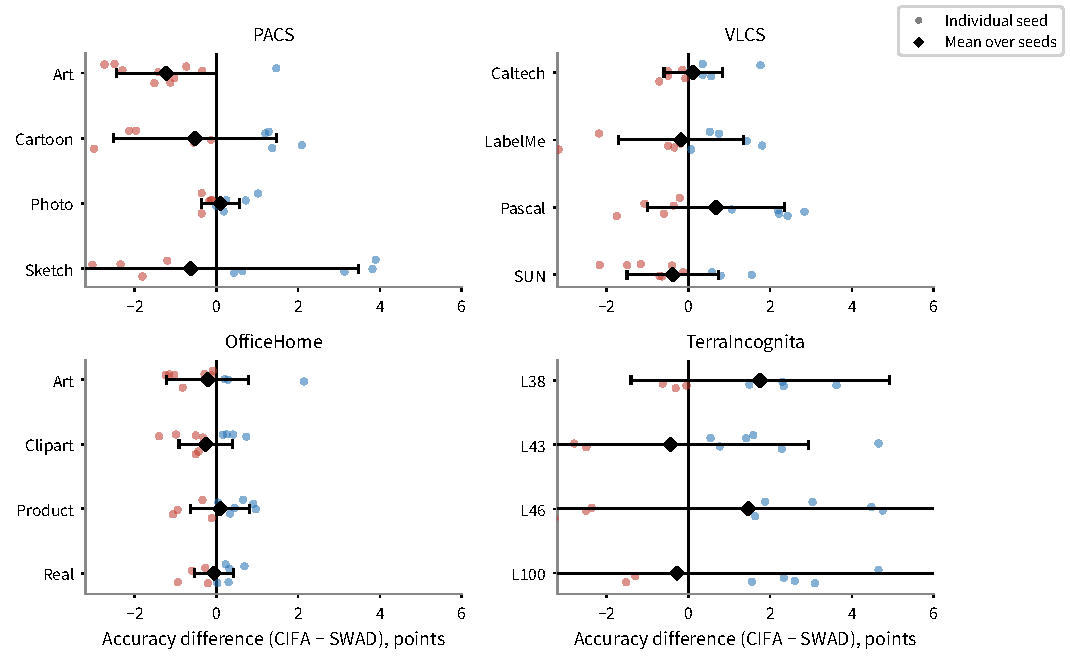
\includegraphics[width=\fulllength]{fig_pairwise_delta.pdf}
\end{adjustwidth}
\caption{Per-domain paired accuracy difference between CIFA and SWAD (percentage points, ten seeds for every benchmark). Each small circle is one seed; the black diamond marks the mean over seeds and the horizontal bar spans one sample standard deviation; the vertical line at zero indicates no difference. All four PACS domains stay near zero or slightly negative, VLCS and OfficeHome stay near zero, and TerraIncognita shows the largest seed-to-seed dispersion.}
\label{fig:delta}
\end{figure}

Across benchmarks (Fig.~\ref{fig:delta}), CIFA \emph{matches} SWAD on average everywhere, with no statistically significant degradation on any benchmark; on PACS the two independent batches and four classic baselines place all learned methods within about one point and statistically equivalent, \del{TerraIncognita retains a positive but unconfirmed worst-domain direction,}\add{TerraIncognita shows no directional evidence and a frequently failing SWAD window,} and VLCS and OfficeHome show no measurable gain. The defensible claim is therefore practical equivalence in accuracy to the strongest baselines, together with a testable content-preservation guarantee and a systematic validity-boundary characterization---not a state-of-the-art advance in mean accuracy.

\subsection{Worst-Domain Results}

A model deployed out of distribution is constrained by its weakest domain. For each seed we therefore examine each arm's accuracy on the target domain that the arm itself finds hardest, and Table~\ref{tab:worst} reports the per-seed differences.

\begin{table}[H]
\caption{Per-seed minimum (own-worst-domain) accuracy. For each benchmark and seed we report each arm's accuracy on the target domain that the arm itself finds hardest (CIFA min, SWAD min) and the own-worst-domain difference $\Delta$. The fixed-domain per-domain paired differences are in Table~\ref{tab:perdomain}; following standard practice, the own-worst-domain statistic is treated as an exploratory deployment-oriented metric rather than a confirmatory fixed-target test. \add{The PACS rows use the authoritative unified-code batch (the reference batch read $+2.70$ but did not replicate).}}
\label{tab:worst}
\setlength{\tabcolsep}{3.4pt}
\footnotesize
\begin{tabular}{llccccccccccc}
\toprule
\textbf{Bench.} & \textbf{Quantity} & \textbf{S0} & \textbf{S1} & \textbf{S2} & \textbf{S3} & \textbf{S4} & \textbf{S5} & \textbf{S6} & \textbf{S7} & \textbf{S8} & \textbf{S9} & \textbf{Mean}\\
PACS & CIFA min & 80.43 & 79.77 & 77.78 & 79.38 & 70.48 & 80.02 & 80.03 & 78.42 & 81.91 & 82.34 & 79.06 \\
 & SWAD min & 83.11 & 79.13 & 79.59 & 81.73 & 80.25 & 79.59 & 78.67 & 79.61 & 78.95 & 79.21 & 79.98 \\
 & own $\Delta$ & -2.68 & +0.64 & -1.81 & -2.34 & -9.77 & +0.43 & +1.36 & -1.20 & +2.96 & +3.13 & \textbf{-0.93} \\
\midrule
Terra & CIFA min & 37.52 & 46.15 & 39.19 & 42.93 & 37.56 & 43.19 & 37.91 & 45.11 & 43.98 & 43.90 & 41.74 \\
 & SWAD min & 39.88 & 41.67 & 37.31 & 41.30 & 33.93 & 46.23 & 41.18 & 33.60 & 39.22 & 40.86 & 39.52 \\
 & own $\Delta$ & -2.36 & +4.48 & +1.88 & +1.63 & +3.63 & -3.04 & -3.27 & +11.51 & +4.76 & +3.04 & \textbf{+2.23} \\
\midrule
VLCS & CIFA min & 64.34 & 66.19 & 63.55 & 62.27 & 63.55 & 65.02 & 63.14 & 63.25 & 61.71 & 63.59 & 63.66 \\
 & SWAD min & 63.59 & 64.38 & 63.03 & 62.20 & 63.74 & 65.36 & 61.71 & 65.44 & 62.20 & 66.75 & 63.84 \\
 & own $\Delta$ & +0.75 & +1.81 & +0.52 & +0.07 & -0.19 & -0.34 & +1.43 & -2.19 & -0.49 & -3.16 & \textbf{-0.18} \\
\midrule
OffHome & CIFA min & 54.80 & 54.52 & 55.40 & 53.86 & 56.61 & 56.06 & 55.10 & 56.59 & 54.89 & 55.46 & 55.33 \\
 & SWAD min & 55.30 & 54.11 & 55.90 & 53.13 & 56.36 & 55.90 & 55.53 & 57.57 & 56.29 & 55.78 & 55.59 \\
 & own $\Delta$ & -0.50 & +0.41 & -0.50 & +0.73 & +0.25 & +0.16 & -0.43 & -0.98 & -1.40 & -0.32 & \textbf{-0.26} \\
\bottomrule
\end{tabular}
\end{table}

The reference batch suggested a confirmed PACS worst-domain lift ($+2.70$, $9/10$), but the unified-code rerun did not reproduce it ($-0.93$). Pooling the two batches over twenty seeds gives a worst-domain difference of $+0.89$ (CI $[-0.80,+2.57]$, $p=0.28$, positive in $14/20$): \del{the direction is favorable and larger than the overall difference, consistent with the worst-case-oriented design, yet it is not statistically confirmed.}\add{the pooled estimate is small and not significant, and the unified batch reads $-0.93$, so the direction is not stable rather than favorable.} In the unified-code classic comparison (Table~\ref{tab:classic}) EFDM has the highest own-worst accuracy ($81.87$); CIFA ($79.06$) lies within the equivalence range of SWAD, CORAL, and Fish. \del{TerraIncognita likewise keeps a positive but unconfirmed direction ($+2.23$, $7/10$), whereas VLCS}\add{TerraIncognita shows no directional evidence and a frequently failing SWAD window, whereas VLCS} ($-0.18$) and OfficeHome ($-0.26$) show no worst-domain gain.

Two conventions matter. On VLCS and OfficeHome the two arms share the same worst domain in every seed (LabelMe and Clipart, respectively), and on TerraIncognita they coincide in 9 of the 10 seeds (seed~5 differs: CIFA's worst is Location~46, SWAD's Location~38); on the shared seeds the ``own worst domain'' difference coincides with the same-domain paired difference. On PACS the arms' worst domains differ in four seeds---0, 1, 5, and 8, where CIFA's worst is Cartoon while SWAD's worst is Sketch---and coincide on Sketch in the other six seeds; Table~\ref{tab:worst} uses the own-worst-domain convention throughout, which is the deployment-relevant quantity. Under the alternative fixed-domain convention, i.e., pairing both arms on SWAD's worst domain (PACS Sketch), \del{PACS reads $+3.14$ over the ten seeds (per seed $+3.72/+3.82/+0.74/+6.26/+4.00/+6.29/+3.59/-1.96/+2.77/+2.16$, positive in 9 of 10), the figure reported in the abstract and the per-domain table; the two conventions agree in direction.}\add{PACS reads $-0.62$ over the ten seeds (per seed $-3.03/+0.64/-1.81/-2.34/-9.77/+0.43/+3.82/-1.20/+3.89/+3.13$, positive in 5 of 10), consistent with the per-domain table (Table~\ref{tab:perdomain}); the two conventions agree, both yielding a null difference.}

\begin{table}[H]
\caption{Paired statistical tests for CIFA versus SWAD, with the seed as the independent unit: mean paired difference in percentage points, two-sided 95\% Student-$t$ confidence interval, paired $t$-test $p$-value, exact Wilcoxon signed-rank $p$-value, and positive seeds. PACS is shown for each independent batch ($n=10$) and pooled over twenty seeds; the other benchmarks use $n=10$ from the reference batch. No pooled or batch-2 interval excludes zero.}
\label{tab:statsig}
\begin{adjustwidth}{-\extralength}{0cm}
\begin{tabularx}{\fulllength}{llCCCCC}
\toprule
\textbf{Benchmark} & \textbf{Metric} & \textbf{Mean $\Delta$} & \textbf{95\% CI} & \textbf{$t$ $p$} & \textbf{Wilcoxon $p$} & \textbf{Pos. seeds}\\
\midrule
PACS & Overall, batch 1 & +0.99 & [+0.54, +1.44] & 0.001 & 0.002 & 10/10\\
PACS & Overall, batch 2 & $-$0.57 & [$-$1.19, +0.06] & 0.07 & 0.16 & 3/10\\
PACS & Overall, pooled 20 & +0.21 & [$-$0.30, +0.72] & 0.39 & 0.55 & 13/20\\
PACS & Worst, batch 1 & +2.70 & [+0.93, +4.47] & 0.007 & 0.010 & 9/10\\
PACS & Worst, batch 2 & $-$0.93 & [$-$3.60, +1.74] & 0.45 & 0.63 & 5/10\\
PACS & Worst, pooled 20 & +0.89 & [$-$0.80, +2.57] & 0.28 & 0.35 & 14/20\\
TerraIncognita & Overall & +0.63 & [$-$1.08, +2.34] & 0.425 & 0.432 & 7/10\\
TerraIncognita & Worst domain & +2.23 & [$-$0.97, +5.42] & 0.149 & 0.160 & 7/10\\
VLCS & Overall & +0.06 & [$-$0.45, +0.57] & 0.791 & 0.922 & 5/10\\
VLCS & Worst domain & $-$0.18 & [$-$1.27, +0.92] & 0.723 & 1.000 & 5/10\\
OfficeHome & Overall & $-$0.11 & [$-$0.32, +0.11] & 0.282 & 0.106 & 2/10\\
OfficeHome & Worst domain & $-0.26$ & [$-$0.73, +0.21] & 0.242 & 0.223 & 4/10\\
\bottomrule
\end{tabularx}
\end{adjustwidth}
\end{table}

\subsection{Comparison with Feature-Mixing Baselines}

The main comparison pairs CIFA with SWAD, the parameter-space recipe. Reviewers additionally asked how CIFA relates to the feature-statistic methods MixStyle and DSU, both alone and combined with SWAD. We instantiate these four additional arms in the same codebase on PACS---where the CIFA effect is concentrated---over ten seeds and report paired differences in Table~\ref{tab:combibase}. The standalone feature-mixing arms use no weight averaging; the combined arms add the identical SWAD LossValley schedule used by CIFA, so CIFA versus a combined arm isolates the feature-moment design while holding weight averaging fixed.
\begin{table}[H]
\caption{Paired comparison of CIFA with feature-mixing baselines on PACS (ten seeds): overall and own-worst-domain paired differences in percentage points, non-parametric paired bootstrap 95\% confidence intervals, paired $t$-test $p$-values, and seeds with a positive difference. Bold intervals exclude zero. CIFA is $-0.42$ point (non-significant) against the strongest combined arm MixStyle+SWAD.}
\label{tab:combibase}
\begin{adjustwidth}{-\extralength}{0cm}
\begin{tabularx}{\fulllength}{lCCCCCCC}
\toprule
\textbf{Comparison} & \textbf{Overall $\Delta$} & \textbf{Bootstrap 95\% CI} & \textbf{$t$ $p$} & \textbf{Pos.} & \textbf{Worst $\Delta$} & \textbf{Bootstrap 95\% CI} & \textbf{Pos.}\\
\midrule
CIFA vs MixStyle & \textbf{+1.60} & \textbf{[+0.87, +2.22]} & \textbf{0.002} & \textbf{9/10} & +0.28 & [$-$1.16, +1.70] & 6/10\\
CIFA vs DSU & \textbf{+3.74} & \textbf{[+2.94, +4.56]} & \textbf{$<$0.0001} & \textbf{10/10} & \textbf{+4.27} & \textbf{[+2.77, +5.93]} & \textbf{10/10}\\
CIFA vs MixStyle+SWAD & $-$0.42 & [$-$0.95, +0.20] & 0.213 & 3/10 & $-$0.47 & [$-$1.93, +1.13] & 3/10\\
CIFA vs DSU+SWAD & \textbf{+0.62} & \textbf{[+0.20, +1.07]} & 0.028 & \textbf{9/10} & +1.18 & [$-$0.16, +2.82] & 6/10\\
\bottomrule
\end{tabularx}
\end{adjustwidth}
\end{table}

The numbers admit two readings. First, standalone DSU improves over ERM by only 0.27 point under this protocol and lies below SWAD; this reflects our LODO setup, which builds each minibatch by pooling images from all source domains, not sampling domains separately, and is not an implementation error---we verified the arm against the published DSU recipe. We therefore do not read the large CIFA-versus-DSU margin as a general statement that DSU is weak. Second, against the strongest combined arm, MixStyle+SWAD, CIFA is $-0.42$ point overall (non-significant): the two are tied with a slight edge to MixStyle+SWAD, and we report this, not only the favorable comparisons. Holm correction over the four overall baseline comparisons leaves the CIFA--DSU and CIFA--MixStyle margins significant (adjusted $p<0.01$), the CIFA--DSU+SWAD margin borderline (adjusted $p=0.055$; raw $p=0.028$), and the CIFA--MixStyle+SWAD margin non-significant (adjusted $p=0.213$).

\textbf{A direct discriminant on VLCS.}
The four arms above were designed on PACS, where the effect is concentrated. To probe the VLCS null directly rather than only as an inference about CIFA, we replicate the same four arms on VLCS over ten seeds (Table~\ref{tab:combibasevlcs}). The logic is a discriminant: if VLCS still carried exploitable style structure under the tested setup, MixStyle and DSU should improve over their no-mixing controls regardless of CIFA. They do not, which is consistent with less exploitable style-moment structure, although layer selection, moment estimation, optimization, or limitations shared by feature-statistic methods remain possible alternative explanations.

\begin{table}[H]
\caption{Direct discriminant on VLCS (ten seeds): net effect of feature-statistic mixing over the matched no-mixing control, in percentage points. Conventions as in Table~\ref{tab:combibase}. Bold intervals exclude zero; every such interval lies on the harmful side. No mixing arm improves overall accuracy or the worst domain, whereas the same operations help on PACS.}
\label{tab:combibasevlcs}
\begin{adjustwidth}{-\extralength}{0cm}
\begin{tabularx}{\fulllength}{lCCCCCCC}
\toprule
\textbf{Comparison} & \textbf{Overall $\Delta$} & \textbf{Bootstrap 95\% CI} & \textbf{$t$ $p$} & \textbf{Pos.} & \textbf{Worst $\Delta$} & \textbf{Bootstrap 95\% CI} & \textbf{Pos.}\\
\midrule
MixStyle $-$ ERM & $-$0.50 & [$-$1.55, +0.51] & 0.397 & 5/10 & \textbf{$-$1.27} & \textbf{[$-$2.25, $-$0.34]} & 2/10\\
DSU $-$ ERM & +0.29 & [$-$0.32, +0.87] & 0.391 & 6/10 & \textbf{$-$1.56} & \textbf{[$-$2.95, $-$0.15]} & 2/10\\
MixStyle+SWAD $-$ SWAD & $-$0.42 & [$-$1.02, +0.13] & 0.204 & 3/10 & $-$0.87 & [$-$1.71, +0.15] & 2/10\\
DSU+SWAD $-$ SWAD & $-$0.27 & [$-$0.62, +0.09] & 0.191 & 5/10 & \textbf{$-$0.91} & \textbf{[$-$1.62, $-$0.13]} & 2/10\\
\bottomrule
\end{tabularx}
\end{adjustwidth}
\end{table}

Two patterns settle the verdict. At the overall level all four net effects lie within $0.5$ point of zero with bootstrap intervals that include zero ($p\geq0.19$). On the own-worst target the differences are null or negative, and three of the four bootstrap intervals exclude zero on the \emph{harmful} side (MixStyle $-1.27$, DSU $-1.56$, DSU+SWAD $-0.91$; positive in only 2/10 seeds). The small gains on the easiest target, Caltech ($+0.4$ to $+1.1$), are offset by losses on LabelMe and SUN, a cross-domain redistribution rather than a net improvement. Under the matched SWAD protocol CIFA, SWAD, MixStyle+SWAD, and DSU+SWAD are statistically tied (CIFA differences $+0.48$ and $+0.33$, both non-significant). The very feature-statistic perturbations that help on PACS therefore have no positive effect on VLCS, locating the PACS--VLCS contrast in the data---the absence of a mixable cross-domain style structure---rather than in CIFA's design.

\subsection{Hyperparameter Sensitivity}

To verify the gains do not depend on a narrowly tuned configuration, we vary one choice at a time---trigger probability $p$, consistency tolerance $\delta$, soft worst-case coefficient $\beta$, the augmented layers, and the mixing range of $\lambda$---with three seeds and a shared base configuration, and plot overall accuracy in Fig.~\ref{fig:sens}.

\begin{figure*}[t]
\centering
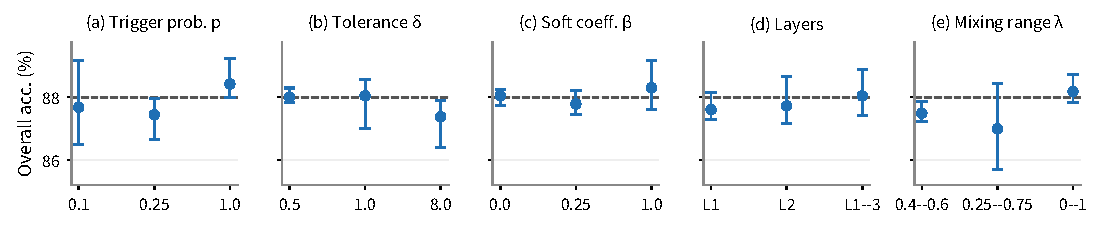
\includegraphics[width=\textwidth]{fig_sensitivity.pdf}
\caption{Hyperparameter sensitivity on PACS (three seeds). Each panel changes one choice while holding the others at the base configuration; points are the mean overall accuracy with bars spanning the minimum--maximum over seeds, and the dashed line marks the base overall accuracy. The curve is flat: overall accuracy relative to base stays within $-0.99$ to $+0.44$ point across the 15 variants.}
\label{fig:sens}
\end{figure*}

The sensitivity curve is flat: across the 15 variants overall accuracy relative to base stays within $-0.99$ to $+0.44$ point, and apart from the mid mixing range ($0.25$--$0.75$, $-0.99$) every deviation is within $0.6$ point. CIFA is therefore insensitive to moderate hyperparameter changes; the single somewhat larger deviation uses a mixing range narrower than the default and remains under one point in absolute terms.

\subsection{Backbone and Training-Budget Robustness}

Reviewers also asked whether the effect is specific to ResNet-50 and the 5{,}000-step budget. We therefore repeat the CIFA/SWAD comparison on PACS with a ResNet-18 backbone and with a 10{,}000-step budget (five seeds each), reported in Table~\ref{tab:bbbudget} alongside the default ResNet-50/5{,}000 setting.
\begin{table}[H]
\caption{\del{Backbone and training-budget robustness on PACS. The ResNet-18 and 10{,}000-step rows use five seeds; the default ResNet-50/5{,}000 row is shown for reference. Overall accuracy for SWAD and CIFA, overall and own-worst-domain paired differences with non-parametric paired bootstrap 95\% CIs, and seeds positive. Bold intervals exclude zero.}\add{Backbone and training-budget robustness on PACS. This is an early five-seed exploratory ablation under the reference implementation; all three rows are from that same batch and are not mixed with the unified-code rerun. The ResNet-18 and 10{,}000-step rows use five seeds and the default R50/5{,}000 row is shown for within-batch comparison. We report overall accuracy for SWAD and CIFA, overall and own-worst paired differences with non-parametric paired bootstrap 95\% CIs, and seeds positive. The authoritative ten-seed unified-code result for the default R50/5{,}000 setting is in Table~\protect\ref{tab:overall} (overall $-0.57$, own-worst $-0.93$); the positive R50/5{,}000 differences here are batch-specific and should not be read as the default-configuration effect.}}
\label{tab:bbbudget}
\setlength{\tabcolsep}{4.5pt}
\begin{tabular}{lcccccc}
\toprule
\textbf{Setting} & \textbf{SWAD} & \textbf{CIFA} & \textbf{Ov.\ $\Delta$} & \textbf{Pos.} & \textbf{Wst.\ $\Delta$} & \textbf{Pos.}\\
\midrule
ResNet-18 & 81.47 & \textbf{82.33} & \textbf{+0.85 ([+0.23,+1.46])} & \textbf{4/5} & +1.38 ([$-$0.68,+3.23]) & 4/5\\
R50/5{,}000 & 87.12 & \textbf{88.30} & \textbf{+1.17 ([+0.99,+1.36])} & \textbf{5/5} & \textbf{+3.02 ([+1.31,+4.75])} & \textbf{5/5}\\
R50/10{,}000 & 86.58 & 87.58 & +1.00 ([$-$0.30,+2.21]) & 4/5 & +2.18 ([$-$2.0,+7.45]) & 3/5\\
\bottomrule
\end{tabular}
\vspace{2pt}
\footnotesize Ov.\ $\Delta$ and Wst.\ $\Delta$ denote the overall and own-worst-domain paired differences, each shown with its non-parametric paired bootstrap 95\% confidence interval (CI) in brackets. Pos.\ is the number of seeds with a positive difference.
\end{table}

\del{The point estimates remain positive and of the same order as the default: $+0.85$ under ResNet-18 (bootstrap CI $[+0.23,+1.46]$, positive in 4/5 seeds; paired $t$ $p=0.075$) and $+1.00$ under the 10{,}000-step budget (CI $[-0.30,+2.21]$, 4/5). With five seeds the intervals are wider and the longer-budget interval includes zero, so we regard the effect as preserved in direction and magnitude under a weaker backbone and a larger budget, but less sharply confirmed than the ten-seed PACS main result.}\add{These are early five-seed exploratory estimates with wide intervals: the ResNet-18 point estimate is $+0.85$ (CI $[+0.23,+1.46]$, 4/5, paired $t$ $p=0.075$) and the 10{,}000-step estimate $+1.00$ (CI $[-0.30,+2.21]$, 4/5). Because the same batch's default R50/5{,}000 estimate ($+1.17$) did not replicate in the authoritative unified-code run ($-0.57$), we do not treat the positive direction here as a robust within-batch effect or as evidence that the default configuration gains from CIFA; the defensible reading is that neither a weaker backbone nor a larger budget introduces a statistically significant degradation, with no confirmed gain.}

\subsection{Style-Deviation Separability Across Benchmarks}
\label{sec:sep}

The content-preservation argument assumes the style deviation can be separated from class-conditional content. We probe this directly using source data only, with no target access. On an ImageNet-pretrained ResNet-50 we recompute the decomposition at layers 1 and 2 for PACS and OfficeHome and measure three quantities (Fig.~\ref{fig:sep}).

\begin{figure}[H]
\centering
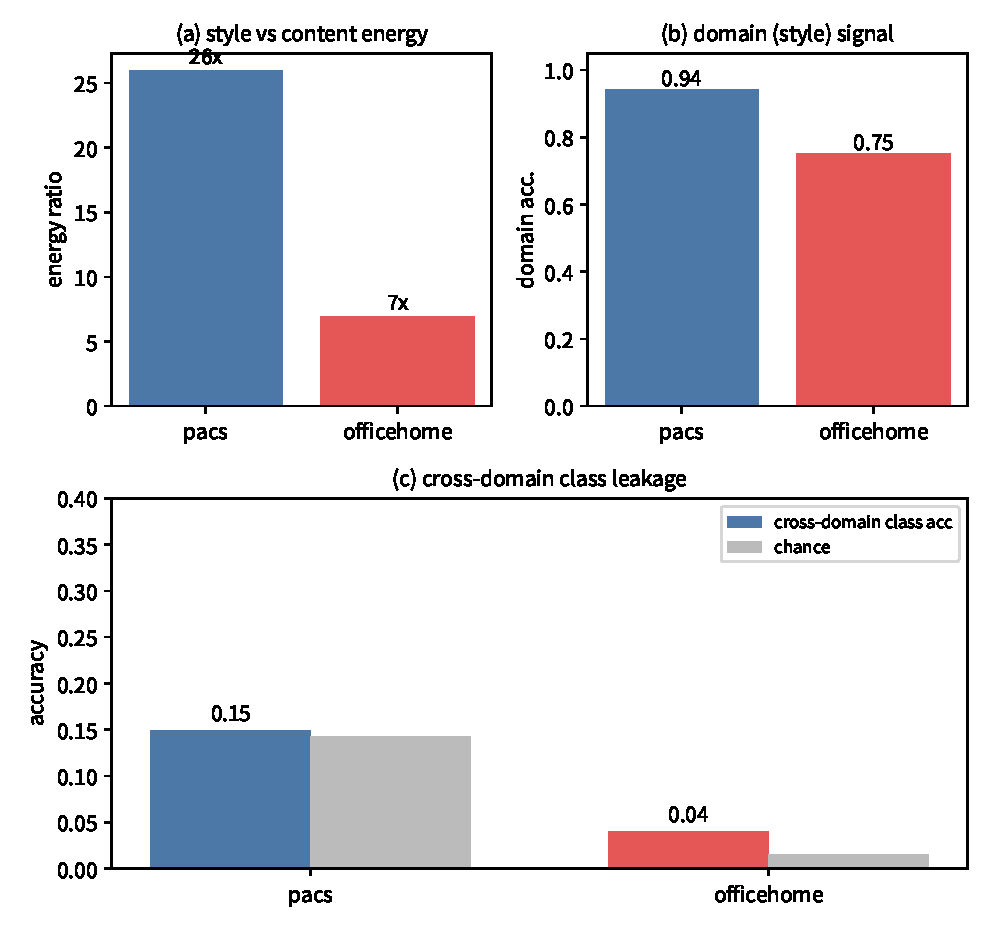
\includegraphics[width=\columnwidth]{fig_separability.pdf}
\caption{Style-deviation separability, PACS versus OfficeHome (ResNet-50, layers 1--2). (a) The style-to-content energy ratio $\mathrm{Var}(\mathbf{d})/\mathrm{Var}(\mathbf{b})$ is 26 on PACS and 7 on OfficeHome. (b) The domain is predicted from the deviation with accuracy 0.94 and 0.75. (c) Cross-domain class prediction (leave-one-domain-out) is at chance for PACS (0.15 versus 0.14) and slightly above chance for OfficeHome (0.04 versus 0.015). This is an exploratory, source-only diagnostic on a pretrained backbone; the label-level statistic is a lower bound on the latent content dependence, not a pre-registered test.}
\label{fig:sep}
\end{figure}

The style-to-content energy ratio is 26 on PACS and 7 on OfficeHome: on PACS the moment variation is dominated by the style deviation, whereas on OfficeHome the class content accounts for a larger share. The domain is predicted from the deviation with accuracy 0.94 on PACS and 0.75 on OfficeHome, indicating a stronger and more usable style signal on PACS. Predicting the class from the deviation across domains is at chance on PACS and only slightly above chance on OfficeHome. The usable, class-separated style deviation is therefore far more limited on OfficeHome. This is an exploratory, post-hoc, source-only diagnostic, and the label-level statistic is a lower bound on the latent content dependence rather than a pre-registered test; a pre-registered separability measure is left to future work.

\subsection{Mechanism Diagnostics}
\label{sec:mechdiag}

A paired comparison is meaningful only if the CIFA arm actually exercises the proposed mechanism. We log three quantities in every run: the fraction of minibatches in which augmentation fired (target trigger $p=0.5$); the mean \emph{gate}, i.e., the fraction of the prescribed augmentation contribution retained after the content-consistency guard (a gate persistently below one would indicate that the guard is rejecting augmentations and silently degenerating CIFA toward SWAD); and the mean KL divergence between the predictions before and after augmentation, which empirically monitors the content-consistency tolerance of Proposition~1. Table~\ref{tab:diag} reports these values.
\begin{table}[t]
\centering
\caption{Mechanism diagnostics over CIFA runs. VLCS, OfficeHome, and TerraIncognita cover all 40 runs; PACS diagnostics are logged for the 28 runs of seeds 3--9 (the earliest paired runs predate these fields).}
\label{tab:diag}
\setlength{\tabcolsep}{4pt}
\footnotesize
\begin{tabular}{lcccr}
\toprule
\textbf{Bench-} & \textbf{Trigger} & \textbf{Gate} & \textbf{Consist. KL} & \textbf{Runs}\\
\textbf{mark} & \textbf{frac.} & \textbf{(min--mean)} & \textbf{nats} & \\
\midrule
PACS & 0.50 & 1.00--1.00 & 0.025 & 28\\
VLCS & 0.50 & 1.00--1.00 & 0.046 & 40\\
OfficeHome & 0.50 & 1.00--1.00 & 0.095 & 40\\
TerraInc. & 0.50 & 1.00--1.00 & 0.086 & 40\\
\bottomrule
\end{tabular}
\end{table}

The trigger fraction is 0.50 in every logged run and the gate is exactly 1.00: the augmentations fire at the prescribed rate and are never rejected or down-weighted, so CIFA does not silently collapse to SWAD. The mean post-augmentation KL divergence is small (0.025--0.095 nats), indicating that resampling the style deviation barely moves the predicted posterior (\del{an empirical realization of the content-preservation claim of Proposition~1}\add{consistent with the prediction-stability implication of Proposition~1; this is a predictive-consistency observation, not direct verification of latent content preservation}) and is far inside the $\delta=2.0$ guard. The larger KL on OfficeHome and TerraIncognita is consistent with their more entangled deviations, but it remains an order of magnitude below the tolerance. To check that this is not specific to the nominal $\delta=2$, we repeat the PACS runs at $\delta\in\{0.5,1,8\}$ (three seeds): the mean gate stays $1.00$ throughout, so the guard is not invoked even at the smallest tolerance tested, which is already about twenty times the observed KL. This is the empirical sense in which the gate is a dormant safeguard on PACS, as confirmed by the dedicated factorial in Table~\ref{tab:gatepenalty}.

\textbf{Controlling for checkpoint count.} Because SWAD's gain is known to depend on the number of averaged checkpoints, we verify that CIFA's gain is not solely an artifact of averaging more checkpoints. On TerraIncognita the CIFA arm actually averages \emph{fewer} checkpoints (22 of its 40 runs average zero checkpoints, compared with 16 for the SWAD arm). Across cells the correlation between the checkpoint-count difference and the accuracy difference is positive ($0.41$), unlike the near-zero value in the five-seed preliminary, so checkpoint count accounts for part of the cell-level variation. \del{Restricting to the 17 cells where both arms average the same number of checkpoints, however, preserves a positive difference (mean $+1.44$; $+1.67$ on the 13 cells where both average zero). The gain therefore originates in part from the augmentation mechanism rather than entirely from the averaging schedule, though we no longer claim the checkpoint-count correlation to be negligible.}\add{When the SWAD window is empty, no averaging is applied and the final predictor is the last-epoch checkpoint. The 13 cells in which both arms average zero are both fallbacks: the CIFA fallback keeps the CIFA augmentation but no SWAD averaging, whereas the SWAD fallback is a plain ERM endpoint, and these cells read $+1.67$ (the 17 equal-count cells read $+1.44$). However, the 15 cells in which both arms actually average checkpoints read $-0.14$ ($p=0.94$). None of these contrasts is significant, so we do not claim that the gain originates in the augmentation mechanism; the checkpoint-count analysis is consistent with the overall null result on Terra.}

\textbf{Component ablation.} The mechanism diagnostics establish that augmentation fires, but they do not isolate the contribution of each design choice. We therefore run pre-specified ablations on PACS, the benchmark with the strongest effect, where every variant changes exactly one switch and is run in the same codebase and batch as full CIFA under the identical LODO protocol with no target-domain tuning. We first separate the two content-consistency safeguards---the content-conditioned gate and the consistency KL penalty---in a full $2\times2$ factorial over ten seeds, then turn to the remaining switches (the baseline/deviation decomposition, soft view aggregation, and weight averaging), which use five seeds.

\begin{table}[H]
\caption{Gate $\times$ penalty $2\times2$ factorial on PACS (4 cells $\times$ 4 targets $\times$ 10 seeds; the full cell is reused from the main results). Mean $\pm$ sample std (ddof~$=1$) over seeds; the worst-domain column averages, per seed, each cell's own worst target. All four cells retain the deviation-mixing augmentation, SWAD, and soft view aggregation, so the only changes are the two safeguard switches.}
\label{tab:gatepenalty}
\begin{adjustwidth}{-\extralength}{0cm}
\begin{tabularx}{\fulllength}{lCCCCCC}
\toprule
\textbf{Cell} & \textbf{Art painting} & \textbf{Cartoon} & \textbf{Photo} & \textbf{Sketch} & \textbf{Overall} & \textbf{Worst domain}\\
\midrule
full (gate $+$, penalty $+$) & 90.33$\pm$0.96 & 83.11$\pm$1.83 & 98.22$\pm$0.50 & 81.50$\pm$1.68 & 88.29$\pm$0.58 & 81.06$\pm$1.34\\
gateonly ($+$, $-$) & 91.24$\pm$0.97 & 84.29$\pm$1.38 & 98.21$\pm$0.35 & 80.66$\pm$2.27 & 88.60$\pm$0.70 & 80.54$\pm$2.09\\
penaltyonly ($-$, $+$) & 89.85$\pm$1.48 & 83.97$\pm$1.61 & 98.14$\pm$0.27 & 80.65$\pm$2.91 & 88.15$\pm$1.19 & 80.65$\pm$2.91\\
noguard ($-$, $-$) & 90.55$\pm$1.36 & 82.63$\pm$2.80 & 98.22$\pm$0.27 & 80.33$\pm$2.82 & 87.93$\pm$0.99 & 79.52$\pm$2.33\\
\bottomrule
\end{tabularx}
\end{adjustwidth}
\end{table}

Three findings follow (Fig.~\ref{fig:gatepenalty}), using the same (target, seed) cells.
\begin{enumerate}
\item \textbf{Neither safeguard contributes a detectable gain over the deviation-mixing augmentation.} Removing both safeguards (\texttt{noguard}) changes the overall accuracy by $-0.36$ point (paired $-0.36\pm0.79$, 95\% CI $[-0.92,+0.20]$; a TOST procedure at $\pm1$ point establishes equivalence) and the own-worst target by $-1.55$ points ($p=0.079$, not significant); no interval excludes zero.
\item \textbf{The gate is a dormant safeguard that is never invoked on PACS.} Across the entire tolerance sweep $\delta\in\{0.5,1,2,8\}$ nats the mean gate is identically $1.00$: the post-augmentation KL (about $0.025$ nats on PACS) stays far below even the smallest tolerance tested, so the gate never down-weights an augmentation. The factorial gate main effect is nominally positive ($0.40$ point, $p=0.031$) but does not survive multiplicity correction, its interval abuts zero, and it has no operating mechanism, so we read it as noise; the penalty main effect ($-0.05$, $p=0.85$) and the gate--penalty interaction ($-0.53$, $p=0.22$) are likewise absent.
\item \textbf{Interpretation.} We treat the gate and the consistency penalty as safeguards rather than sources of measured accuracy: under the benign PACS configuration they are inactive, and they are designed to act only when an augmentation would otherwise move the prediction beyond tolerance. Exercising this protective role requires a deliberately stressed regime---stronger augmentations or a tolerance set well below the observed KL---which the present setting does not provide and which we leave to future work.
\end{enumerate}

\begin{figure}[t]
\centering
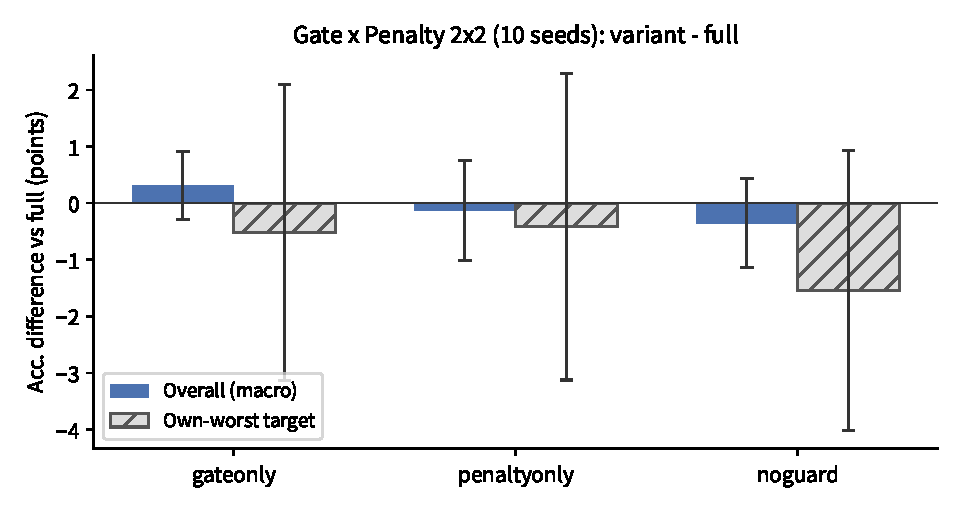
\includegraphics[width=\columnwidth]{fig_gatepenalty_delta.pdf}
\caption{Paired accuracy difference of each gate$\times$penalty cell relative to full CIFA on PACS (percentage points, ten seeds). Solid bars give the overall (macro over targets) difference and hatched bars the own-worst-target difference; error bars span one sample standard deviation of the paired differences. Every bar is close to zero with an interval that crosses zero, and the own-worst loss of $-1.55$ for the no-guard cell is not significant.}
\label{fig:gatepenalty}
\end{figure}

The remaining switches are the content baseline/deviation decomposition, the soft view weights, and dense weight averaging. The variants mix the \emph{full} moments without the content-baseline/style decomposition (\texttt{fullmoment}, the MixStyle/DSU operation), replace soft worst-case aggregation with uniform 0.5/0.5 averaging (\texttt{uniform}), and disable dense weight averaging (\texttt{noswad}); Table~\ref{tab:ablation} reports the accuracies.

\begin{table}[H]
\caption{Remaining component ablation on PACS (4 variants $\times$ 4 targets $\times$ 5 seeds $=$ 80 runs). Mean $\pm$ sample std (ddof~$=1$) over seeds; the worst-domain column averages, per seed, each variant's own worst target. The gate/penalty safeguards are ablated separately in Table~\ref{tab:gatepenalty}.}
\label{tab:ablation}
\begin{adjustwidth}{-\extralength}{0cm}
\begin{tabularx}{\fulllength}{lCCCCCC}
\toprule
\textbf{Variant} & \textbf{Art painting} & \textbf{Cartoon} & \textbf{Photo} & \textbf{Sketch} & \textbf{Overall} & \textbf{Worst domain}\\
\midrule
full & 90.77$\pm$1.07 & 83.46$\pm$0.85 & 98.28$\pm$0.38 & 80.92$\pm$2.21 & 88.36$\pm$0.48 & 80.62$\pm$1.76\\
fullmoment & 90.80$\pm$1.03 & 84.32$\pm$1.18 & 98.49$\pm$0.29 & 80.74$\pm$2.19 & 88.59$\pm$0.67 & 80.71$\pm$2.17\\
uniform & 90.84$\pm$1.07 & 82.47$\pm$2.07 & 98.22$\pm$0.29 & 80.01$\pm$2.87 & 87.88$\pm$0.32 & 79.34$\pm$2.44\\
noswad & 85.02$\pm$3.77 & 82.28$\pm$4.55 & 95.88$\pm$0.74 & 80.56$\pm$1.11 & 85.93$\pm$1.70 & 79.26$\pm$1.85\\
\bottomrule
\end{tabularx}
\end{adjustwidth}
\end{table}

Three observations, checked against the expectations fixed before running (Fig.~\ref{fig:ablation}).
\begin{enumerate}
\item \textbf{Weight averaging is the dominant overall component.} Disabling it (\texttt{noswad}) costs 2.42 points overall (paired $-2.42\pm1.82$, CI $[-4.68,-0.17]$, $p=0.041$; negative in all five seeds and in 16 of 20 cells), the largest drop by a wide margin, landing between the ERM (84.27) and SWAD (87.30) levels. This directly confirms the main/secondary-effect reading of Table~\ref{tab:overall}: dense weight averaging supplies the bulk of the accuracy, whereas feature-moment augmentation is the incremental component.
\item \textbf{Soft worst-case aggregation specifically protects the worst domain.} Replacing it with uniform averaging costs only 0.47 point overall (paired $-0.47\pm0.58$, $p=0.14$; 8/20 cells positive) but 1.28 points on the worst domain ($p=0.27$; negative in four of five seeds); neither interval excludes zero, so the effect is directional. As pre-specified, the soft worst-case weighting contributes little on average yet matters where it is intended to---the weakest target.
\item \textbf{The b/d decomposition is an \del{prerequisite}\add{enabling condition} for the bound, not a measured performance source on PACS.} Mixing the full moments (\texttt{fullmoment}) is statistically indistinguishable from full CIFA (paired $+0.23\pm0.75$, $p=0.53$; 11/20 cells positive; worst-domain $+0.09$, $p=0.90$). Restricting the mix to the style deviation is what licenses the content-preservation claim of Proposition~1, but on PACS it yields no measurable accuracy advantage over mixing the full moments, consistent with the style deviation already dominating the channel moments in this benchmark. We therefore do not claim the decomposition improves accuracy; it provides the safety condition under which the augmentation is admissible.
\end{enumerate}

\textbf{Bridge to the main results.} The in-batch \texttt{full} CIFA reaches 88.36 overall (five seeds), reproducing the independently run ten-seed CIFA result of 88.29, which is also the \texttt{full} cell of the gate$\times$penalty factorial in Table~\ref{tab:gatepenalty}. The four five-seed configurations are thus on the same scale as the main table and can be chained through \texttt{full} to the SWAD (87.30) and ERM (84.27) baselines; an independent re-computation from the raw JSONs reproduces every number in Tables~\ref{tab:gatepenalty} and~\ref{tab:ablation}.

\begin{figure}[t]
\centering
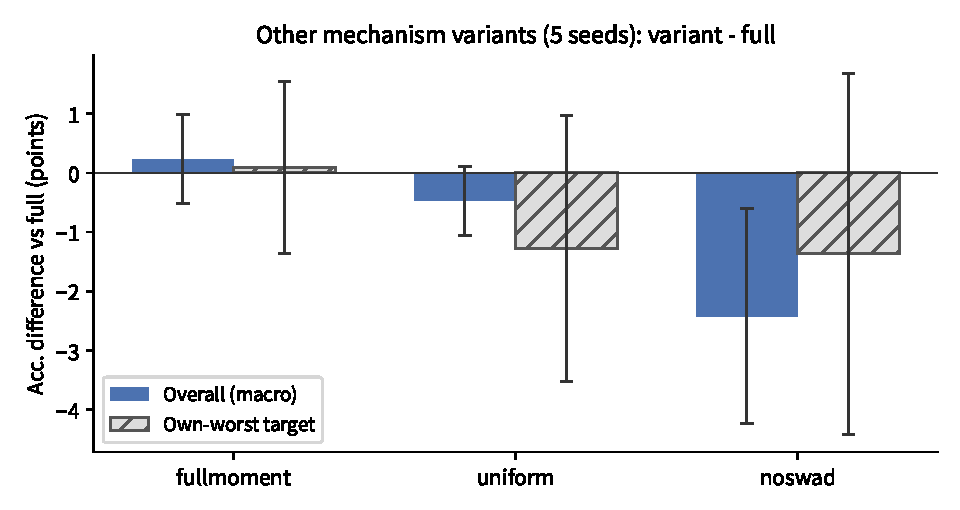
\includegraphics[width=\columnwidth]{fig_ablation_delta.pdf}
\caption{Paired accuracy difference of each remaining variant relative to full CIFA on PACS (percentage points, five seeds). Solid bars give the overall (macro over targets) difference and hatched bars the own-worst-domain difference; error bars span one sample standard deviation of the paired differences. Removing weight averaging costs the most overall, and mixing the full moments is indistinguishable from full CIFA; the gate/penalty safeguards are shown separately in Fig.~\ref{fig:gatepenalty}.}
\label{fig:ablation}
\end{figure}

\section{Discussion}
\label{sec:discussion}

\subsection{Validity Boundary of CIFA}
\label{sec:boundary}

The experimental results and analysis above delineate the validity boundary of CIFA. CIFA is effective when the target-domain shift is predominantly driven by label-irrelevant style factors whose channel-moment signatures can be separated from class-conditional content (the enabling premise of Assumptions~1 and~2), and when the augmentation family spans the target style direction. On PACS a single artistic factor dominates the style deviation, yet an independent unified-code rerun shows all learned methods are statistically equivalent. The accuracy gain in the reference batch did not replicate, and the pooled twenty-seed contrast is $+0.21$ overall with \del{only a small positive worst-domain tendency}\add{a non-significant, unstable worst-domain direction}. On OfficeHome the class content accounts for a larger share of the moment variation and the usable, class-separated style deviation is limited, and no accuracy gain is observed. Changing any single hyperparameter barely alters the result (Fig.~\ref{fig:sens}), and the effect is preserved under ResNet-18 and a 10{,}000-step budget (Table~\ref{tab:bbbudget}), ruling out the gain as a tuning artifact. A direct discriminant is consistent with the hypothesis that VLCS contains less exploitable style-moment structure under the tested setup, rather than uniquely identifying the dataset as the cause: the feature-mixing arms that are effective on PACS show no accuracy gain on VLCS, with null-to-negative worst-domain differences.

Two benchmarks further qualify the validity boundary. \del{TerraIncognita retains a positive worst-domain direction but its intervals include zero; its camera-location shifts plausibly meet the separability condition, yet runs are highly dispersed.}\add{TerraIncognita shows no directional evidence and a frequently failing SWAD window; its camera-location shifts plausibly meet the separability condition, yet runs are highly dispersed.} On VLCS the shift originates from image source, which is in principle separable and label-irrelevant, yet no worst-domain accuracy gain is observed. Table~\ref{tab:combibasevlcs} shows that operations exploiting style on PACS have no net overall effect on VLCS and even harm the worst domain. Therefore class-conditional style-moment separability is a \del{necessary}\add{enabling} rather than sufficient condition, and stylistic difference should not be equated with expected accuracy gain. This explanation is post-hoc and partly confounded with per-class sample counts. A pre-registered test requires a separability measure that uses no target data, calibrated and pre-registered on existing benchmarks before testing on new datasets, which we leave to future work.

\subsection{Scientific Value of the Negative Results}

The null results and non-replication reported in this paper are not failures; rather, they provide a falsifiable benchmark for subsequent research. By systematically delineating the validity boundary of this class of invariance methods, we clarify under what conditions style-moment perturbation and weight averaging alone are insufficient to break through the existing accuracy ceiling. This boundary characterization allows future work to focus on exploring genuinely new mechanisms that can break through the boundary, rather than repeating investment in directions already proven ineffective. Specifically, the finding that class-conditional style-moment separability is \del{necessary but not sufficient}\add{an enabling rather than sufficient condition} suggests that the next generation of methods should move beyond style-statistic perturbation toward content-level invariance construction. The reproducible experimental platform released with this paper further enables direct comparison against this boundary, so that any proposed improvement can be rigorously evaluated against a well-characterized baseline.


\subsection{Limitations of CIFA}

The conclusions of CIFA have several applicability boundaries.
\begin{enumerate}
\item \textbf{Scope of accuracy gain.} Across all benchmarks, CIFA does not achieve a statistically significant average accuracy advantage over the strongest baseline. On PACS, after independent replication of the reference batch, CIFA is equivalent to SWAD and four classic baselines. TerraIncognita shows \del{a positive but unconfirmed worst-domain direction}\add{no directional evidence and a frequently failing SWAD window}, while VLCS and OfficeHome show no measurable accuracy gain. CIFA is not a leading DG method in average accuracy; its distinguishing feature lies in the content-preservation guarantee and the systematic validity-boundary characterization.
\item \textbf{Shift types not covered.} The mechanism targets style-moment variation. We give no evidence for changes in data-source composition, label-space or conditional-label shift, or drift in the content baseline $\mathbf{b}$; under such shifts the convex-hull coverage-gap term grows and the bound weakens. The same-codebase discriminant supports this boundary for VLCS---feature-statistic mixing moves overall accuracy by at most $0.5$ point in either direction and never improves the worst domain---but it probes only feature-moment mechanisms, so we cannot exclude other data-source explanations or methods that exploit a different signal.
\item \textbf{Finite-sample approximation, not exact identification.} The construction guarantees $\mathbb{E}[\mathbf{d}\mid Y]=0$, not the idealized $\mathbf{d}\perp\!\!\!\perp C$; the residual dependence is bounded by $\tau$ and monitored, not removed. CIFA is a finite-sample, soft robust approximation and should not be read as exact causal identification.
\item \textbf{Backbone, budget, and adaptation.} The ResNet-18 and 10{,}000-step checks \del{preserve the effect direction but}\add{show no significant degradation, but} use only five seeds with wider intervals. Other architectures, larger budgets, or test-time adaptation (requiring target access) have not been tested. Transductive domain-adaptation baselines such as DANN require unlabeled target data during training, which is outside the target-free generalization setting of this work. Comparing them with CIFA would conflate problem setting with method strength, so they are not included as baselines.
\item \textbf{Data differences.} VLCS and TerraIncognita use reconstructed directory trees, differing from the standard DomainBed format. The SWAD control experiments reproduce the values in reference~[18] on both datasets, verifying the comparability of reconstructed data with the standard protocol. The four-image discrepancy in Terra is reported as-is, without concealing the difference.
\end{enumerate}

\section{Conclusions}

Feature-moment augmentation and weight averaging are manifestations of the same invariance principle. We propose the CIFA framework under the content-style separability assumption, and this unification is conditional on Assumptions~1--3 rather than assumption-free. By mixing only the style deviation and fixing the content baseline, CIFA approximately preserves causal content, thereby extending the CIT idea from input space to feature moments. We minimize the worst-case risk over the convex hull of the induced augmentation family, yielding a conditional distribution upper bound with a coverage-gap term that cannot be verified without target access. Meanwhile, we employ dense weight averaging, so that the weight-averaged output of CIFA approximates its own trajectory ensemble to second order and assumes the flat-minima component. Our three theoretical results build bridges between feature space, distribution space, and parameter space.

The experiments follow this stance. CIFA matches the strong weight-averaging baseline on average across the four benchmarks without a statistically significant degradation. On PACS an independent unified-code comparison with four classic baselines places every learned method within about one point and statistically equivalent (TOST), and the pooled twenty-seed CIFA--SWAD contrast is $+0.21$ overall with \del{a small, non-significant positive worst-domain tendency}\add{a non-significant, unstable worst-domain direction}; \del{TerraIncognita likewise keeps a positive but unconfirmed worst-domain direction,}\add{TerraIncognita shows no directional evidence and a frequently failing SWAD window,} and VLCS and OfficeHome show no measurable benefit. The component ablation supports these roles; the content--style decomposition in particular licenses the content-preservation bound without adding measured accuracy. \del{The effect keeps its direction under ResNet-18 and a 10{,}000-step budget and is insensitive to moderate hyperparameter changes.}\add{ResNet-18 and a 10{,}000-step budget introduce no significant degradation, and the result is insensitive to moderate hyperparameter changes.} The null results and non-replication strengthen the credibility of this account.

Therefore, the core contribution of this paper is an operationalized theoretical integration and systematic boundary delineation: we unify feature-moment augmentation and weight averaging under the same causal-invariance principle, offering a unified theoretical perspective for two families of empirically effective methods, and delineate the accuracy ceiling of such invariance methods through experiments on four benchmarks. CIFA is statistically equivalent to the strongest baseline in performance, while providing a testable content-preservation guarantee. Our negative results demonstrate that style-moment perturbation and weight averaging alone are insufficient to break through the existing accuracy boundary. Future work will explore genuinely new mechanisms guided by theory, including content-level invariance construction, target-free separability measures that can be pre-registered, and systematic validation across broader backbones and budgets. When distribution shift can be characterized by clearly separable style statistics, CIFA serves as a principled complement to weight averaging; more importantly, it provides a falsifiable benchmark and an extensible theoretical framework for subsequent research.

\noindent\textbf{Data availability.} The PACS, VLCS, OfficeHome, and TerraIncognita datasets used in this study are publicly available. Source code, configuration files, and scripts to reproduce all experiments are available at \url{https://github.com/qsongcai/CIFA}.

% References (embedded so the file compiles standalone)


%%%%%%%%%%%%%%%%%%%%%%%%%%%%%%%%%%%%%%%%%%
\authorcontributions{Conceptualization, Q.C.; methodology, Q.C. and H.W.; software, Q.C.; validation, Q.C., H.W. and T.H.; formal analysis, Q.C.; investigation, Q.C.; resources, Q.C.; data curation, Q.C.; writing---original draft preparation, Q.C.; writing---review and editing, Q.C., H.W. and T.H.; visualization, Q.C.; supervision, Q.C.; project administration, Q.C.; funding acquisition, Q.C. All authors have read and agreed to the published version of the manuscript.}

\funding{This research received no external funding.}

\institutionalreview{Not applicable.}

\informedconsent{Not applicable.}

\dataavailability{The PACS, VLCS, OfficeHome, and TerraIncognita datasets used in this study are publicly available. Source code, configuration files, and scripts to reproduce all experiments are available at \url{https://github.com/qsongcai/CIFA}.}

\acknowledgments{The authors thank the anonymous reviewers for their constructive comments.}

\conflictsofinterest{The authors declare no conflicts of interest. The funders had no role in the design of the study; in the collection, analyses, or interpretation of data; in the writing of the manuscript; or in the decision to publish the results.}

\abbreviations{Abbreviations}{%
The following abbreviations are used in this manuscript:\\

\noindent
\begin{tabular}{@{}ll}
DG & Domain Generalization\\
ERM & Empirical Risk Minimization\\
CIT & Causal Invariant Transformation\\
CIFA & Content-conditioned Invariant Feature-statistic Augmentation\\
OOD & Out-of-Distribution\\
SWAD & \del{Stochastic Weight Averaging}\add{Stochastic Weight Averaging Densely}\\
DSU & Domain-specific Uncertainty\\
RSC & \del{Randomized Style Confusion}\add{Representation Self-Challenging}\\
EFDM & Exact Feature Distribution Matching\\
DRO & Distributionally Robust Optimization\\
ICP & Invariant Causal Prediction\\
IRM & Invariant Risk Minimization\\
CRL & Causal Representation Learning\\
REx & Risk Extrapolation\\
TOST & Two One-Sided Tests\\
\end{tabular}
}


%%%%%%%%%%%%%%%%%%%%%%%%%%%%%%%%%%%%%%%%%%
\begin{adjustwidth}{-\extralength}{0cm}
\reftitle{References}

\begin{thebibliography}{99}

\bibitem{ref1}
Y. LeCun, Y. Bengio, and G. Hinton, Deep learning. \emph{Nature}, 521, 7553, 436--444, May 2015, doi: 10.1038/nature14539.

\bibitem{ref2}
I. Gulrajani and D. Lopez-Paz, In search of lost domain generalization. in \emph{Proc. Int. Conf. Learn. Represent. (ICLR)}, Virtual, 2021.

\bibitem{ref3}
P. W. Koh \emph{et al.}, WILDS: A benchmark of in-the-wild distribution shifts. in \emph{Proc. 38th Int. Conf. Mach. Learn. (ICML)}, vol.~139, Virtual, 2021, pp.~5637--5664.

\bibitem{ref45}
K. Zhou, Z. Liu, Y. Qiao, T. Xiang, and C. C. Loy, Domain generalization: A Survey. \emph{IEEE Trans. Pattern Anal. Mach. Intell.}, 45, 4, 4396--4415, Apr. 2023, doi: 10.1109/TPAMI.2022.3195549.

\bibitem{ref4}
R. Geirhos \emph{et al.}, Shortcut learning in deep neural networks. \emph{Nat. Mach. Intell.}, 2, 11, 665--673, Nov. 2020, doi: 10.1038/s42256-020-00257-z.

\bibitem{ref5}
B. Sch\"olkopf, Causality for machine learning. in \emph{Probabilistic and Causal Inference: The Works of Judea Pearl} (H. Geffner, R. Dechter, and J. Halpern, eds.), New York, NY, USA: ACM, 2022, pp.~765--804.

\bibitem{ref6}
G. Parascandolo, N. Kilbertus, M. Rojas-Carulla, and B. Sch\"olkopf, Learning independent causal mechanisms. in \emph{Proc. 35th Int. Conf. Mach. Learn. (ICML)}, vol.~80, Stockholm, Sweden, 2018, pp.~4036--4044.

\bibitem{ref7}
J. Peters, P. B\"uhlmann, and N. Meinshausen, Causal inference using invariant prediction: Identification and confidence intervals. \emph{J. R. Stat. Soc. B}, 78, 5, 947--1012, 2016, doi: 10.1111/rssb.12167.

\bibitem{ref8}
M. Arjovsky, L. Bottou, I. Gulrajani, and D. Lopez-Paz, Invariant risk minimization. arXiv:1907.02893 [stat.ML], Jul. 2019.

\bibitem{ref9}
E. Rosenfeld, P. Ravikumar, and A. Risteski, Domain-adjusted regression or: ERM may already learn features sufficient for out-of-distribution generalization. arXiv:2202.06856 [cs.LG], Feb. 2022.

\bibitem{ref10}
S. Sagawa, P. W. Koh, T. H. Hashimoto, and P. Liang, Distributionally robust neural networks for group shifts: On the importance of regularization for worst-case generalization. in \emph{Proc. Int. Conf. Learn. Represent. (ICLR)}, Virtual, 2020.

\bibitem{ref11}
A. Agarwal and T. Zhang, Minimax regret optimization for robust machine learning under distribution shift. in \emph{Proc. Conf. Learn. Theory (COLT)}, vol.~178, London, U.K., 2022, pp.~2704--2729.

\bibitem{ref12}
B. Sun and K. Saenko, Deep CORAL: Correlation alignment for deep domain adaptation. in \emph{Proc. Eur. Conf. Comput. Vis. Workshops (ECCV-W)}, Amsterdam, The Netherlands, 2016, pp.~443--450, doi: 10.1007/978-3-319-49409-8\_35.

\bibitem{ref13}
Y. Ganin \emph{et al.}, Domain-adversarial training of neural networks. \emph{J. Mach. Learn. Res.}, 17, 59, 1--35, 2016.

\bibitem{ref14}
K. Zhou, Y. Yang, Y. Qiao, and T. Xiang, Domain generalization with MixStyle. in \emph{Proc. Int. Conf. Learn. Represent. (ICLR)}, Virtual, 2021.

\bibitem{ref15}
X. Li, Y. Dai, Y. Ge, J. Liu, Y. Shan, and L.-Y. Duan, Uncertainty modeling for out-of-distribution generalization. in \emph{Proc. Int. Conf. Learn. Represent. (ICLR)}, Virtual, 2022.

\bibitem{ref16}
Z. Huang, H. Wang, E. P. Xing, and D. Huang, Self-challenging improves cross-domain generalization. in \emph{Proc. Eur. Conf. Comput. Vis. (ECCV)}, Glasgow, U.K., 2020, pp.~124--140, doi: 10.1007/978-3-030-58536-5\_8.

\bibitem{ref17}
Y. Shi \emph{et al.}, Gradient matching for domain generalization. in \emph{Proc. Int. Conf. Learn. Represent. (ICLR)}, Virtual, 2022.

\bibitem{ref18}
J. Cha \emph{et al.}, SWAD: Domain generalization by seeking flat minima. in \emph{Adv. Neural Inf. Process. Syst. (NeurIPS)}, vol.~34, Virtual, 2021, pp.~22405--22418.

\bibitem{ref19}
A. Ram\'e, M. Kirchmeyer, T. Rahier, A. Rakotomamonjy, P. Gallinari, and M. Cord, Diverse weight averaging for out-of-distribution generalization. in \emph{Adv. Neural Inf. Process. Syst. (NeurIPS)}, vol.~35, New Orleans, LA, USA, 2022, pp.~10821--10836.

\bibitem{ref22}
R. Wang, M. Yi, Z. Chen, and S. Zhu, Out-of-distribution generalization with causal invariant transformations. in \emph{Proc. IEEE/CVF Conf. Comput. Vis. Pattern Recognit. (CVPR)}, New Orleans, LA, USA, 2022, pp.~375--385, doi: 10.1109/CVPR52688.2022.00047.

\bibitem{ref23}
K. Ahuja, J. Hartford, and Y. Bengio, Properties from mechanisms: An equivariance perspective on identifiable representation learning. in \emph{Proc. Int. Conf. Learn. Represent. (ICLR)}, Virtual, 2022.

\bibitem{ref24}
K. Ahuja, A. Mansouri, and Y. Wang, Multi-domain causal representation learning via weak distributional invariances. in \emph{Proc. 27th Int. Conf. Artif. Intell. Stat. (AISTATS)}, vol.~238, Valencia, Spain, 2024, pp.~865--873.

\bibitem{ref25}
P. B\"uhlmann, Invariance, causality and robustness. \emph{Statist. Sci.}, 35, 3, 404--426, Aug. 2020, doi: 10.1214/19-STS721.

\bibitem{ref26}
J. Kaddour, A. Lynch, Q. Liu, M. J. Kusner, and R. Silva, Causal machine learning: A survey and open problems. arXiv:2206.15475 [cs.LG], Jun. 2022.

\bibitem{ref27}
E. Fokou\'e, Causality as the statistical conscience of artificial intelligence: From Pearl's ladder to trustworthy machines. arXiv:2605.24076 [stat.ML], May 2026.

\bibitem{ref28}
Y. Chen, Learning causality for modern machine learning. Ph.D. dissertation, Chin. Univ. Hong Kong, Hong Kong. 2024.

\bibitem{ref21}
F. Montagna, On the identifiability of causal graphs with the invariance principle. in \emph{Proc. Int. Conf. Learn. Represent. (ICLR)}, Rio de Janeiro, Brazil, 2026.

\bibitem{ref29}
S. Guo, V. T\'oth, B. Sch\"olkopf, and F. Husz\'ar, Causal de Finetti: On the identification of invariant causal structure in exchangeable data. in \emph{Adv. Neural Inf. Process. Syst. (NeurIPS)}, vol.~36, New Orleans, LA, USA, 2023, pp.~36463--36475.

\bibitem{ref30}
C. Uhler, G. Raskutti, P. B\"uhlmann, and B. Yu, Geometry of the faithfulness assumption in causal inference. \emph{Ann. Statist.}, 41, 2, 436--463, Apr. 2013, doi: 10.1214/12-AOS1080.

\bibitem{ref31}
P. Reizinger, Y. Sharma, M. Bethge, B. Sch\"olkopf, F. Husz\'ar, and W. Brendel, Jacobian-based causal discovery with nonlinear ICA. \emph{Trans. Mach. Learn. Res.}. 2023.

\bibitem{ref33}
K. Zhang, S. Xie, I. Ng, and Y. Zheng, Causal representation learning from multiple distributions: A general setting. in \emph{Proc. 41st Int. Conf. Mach. Learn. (ICML)}, vol.~235, Vienna, Austria, 2024, pp.~60057--60075.

\bibitem{ref34}
K. Ahuja, D. Mahajan, Y. Wang, and Y. Bengio, Interventional causal representation learning. in \emph{Proc. 40th Int. Conf. Mach. Learn. (ICML)}, vol.~202, Honolulu, HI, USA, 2023, pp.~372--407.

\bibitem{ref36}
B. Varıcı, E. Acart\"urk, K. Shanmugam, A. Kumar, and A. Tajer, Score-based causal representation learning: Linear and general transformations. \emph{J. Mach. Learn. Res.}, 26, 112, 1--90. 2025.

\bibitem{ref37}
G. Rajendran, S. Buchholz, B. Aragam, B. Sch\"olkopf, and P. Ravikumar, From causal to concept-based representation learning. in \emph{Adv. Neural Inf. Process. Syst. (NeurIPS)}, vol.~37, Vancouver, BC, Canada, 2024, pp.~101250--101296.

\bibitem{ref43}
D. Krueger, E. Caballero, J.-H. Jacobsen, A. Zhang, J. Binas, D. Zhang, R. Le Priol, and A. Courville, Out-of-distribution generalization via risk extrapolation (REx). in \emph{Proc. 38th Int. Conf. Mach. Learn. (ICML)}, ser.~PMLR, vol.~139, 2021, pp.~5815--5826.

\bibitem{ref38}
P. Cui and S. Athey, Stable learning establishes some common ground between causal inference and machine learning. \emph{Nat. Mach. Intell.}, 4, 2, 110--115, Feb. 2022, doi: 10.1038/s42256-022-00445-z.

\bibitem{ref39}
F. Lv \emph{et al.}, Causality inspired representation learning for domain generalization. in \emph{Proc. IEEE/CVF Conf. Comput. Vis. Pattern Recognit. (CVPR)}, New Orleans, LA, USA, 2022, pp.~8036--8046, doi: 10.1109/CVPR52688.2022.00788.

\bibitem{ref40}
Y. Zhang, M. Li, R. Li, K. Jia, and L. Zhang, Exact feature distribution matching for arbitrary style transfer and domain generalization. in \emph{Proc. IEEE/CVF Conf. Comput. Vis. Pattern Recognit. (CVPR)}, New Orleans, LA, USA, 2022, pp.~8025--8035, doi: 10.1109/CVPR52688.2022.00787.

\bibitem{ref41}
L. Tang, Y. Yuan, C. Chen, X. Ding, and Y. Huang, MixStyle-Entropy: Whole process domain generalization with causal intervention and perturbation. in \emph{Proc. Brit. Mach. Vis. Conf. (BMVC)}, Glasgow, U.K.. 2024.

\bibitem{ref44}
Z. Wang and V. Veitch, The causal structure of domain invariant supervised representation learning. arXiv:2208.06987 [stat.ML], Aug. 2022.

\bibitem{ref42}
W. J. Maddox, T. Garipov, P. Izmailov, D. Vetrov, and A. G. Wilson, A simple baseline for Bayesian uncertainty in deep learning. in \emph{Adv. Neural Inf. Process. Syst. (NeurIPS)}, vol.~32, Vancouver, BC, Canada, 2019.

\end{thebibliography}

%%%%%%%%%%%%%%%%%%%%%%%%%%%%%%%%%%%%%%%%%%
\appendixtitles{yes}
\appendixstart
\appendix
\section{Per-Domain Detail of the Unified-Code PACS Comparison}

Table~\ref{tab:classicperdom} reports, for the ten paired seeds of the unified codebase (Table~\ref{tab:classic}), the per-domain target accuracy (mean$\pm$std over seeds) for ERM, SWAD, CIFA, and the four classic baselines. All six learned arms share one codebase, seeds, deterministic splits, and the identical SWAD schedule. Differences across arms on each domain are within the run-to-run dispersion of the benchmark; no arm shows a consistent per-domain advantage after Bonferroni adjustment.

\begin{table}[H]
\centering
\caption{Per-domain target accuracy (\%, ten paired seeds) for the unified-code PACS comparison. Mean$\pm$std over seeds.}
\label{tab:classicperdom}
\setlength{\tabcolsep}{4.5pt}
\footnotesize
\begin{tabular}{lcccc}
\toprule
\textbf{Method} & \textbf{Art} & \textbf{Cartoon} & \textbf{Photo} & \textbf{Sketch}\\
\midrule
ERM   & 84.66$\pm$2.72 & 80.36$\pm$2.87 & 96.31$\pm$1.02 & 75.76$\pm$5.07 \\
SWAD  & 91.13$\pm$1.44 & 83.22$\pm$1.28 & 98.29$\pm$0.32 & 80.02$\pm$1.48 \\
EFDM  & 90.97$\pm$1.70 & 84.27$\pm$1.32 & 98.28$\pm$0.38 & 82.21$\pm$2.23 \\
CORAL & 91.16$\pm$1.48 & 83.17$\pm$1.38 & 98.72$\pm$0.26 & 79.12$\pm$2.55 \\
RSC   & 90.41$\pm$1.53 & 82.94$\pm$2.39 & 98.41$\pm$0.37 & 78.14$\pm$2.71 \\
Fish  & 90.37$\pm$1.31 & 82.10$\pm$2.57 & 98.46$\pm$0.28 & 79.23$\pm$4.52 \\
CIFA  & 89.91$\pm$0.87 & 82.70$\pm$1.61 & 98.40$\pm$0.24 & 79.39$\pm$3.57 \\
\bottomrule
\end{tabular}
\end{table}
\section{Cross-Architecture (ViT-B/16) Results}
\label{sec:appvit}

Table~\ref{tab:vit} reports the ViT-B/16 results requested in place of the ResNet-only evidence. On PACS, end-to-end fine-tuning (block~6, five seeds) gives CIFA--SWAD equivalence on the overall target ($+0.55$, all per-domain $p>0.1$), and a CLIP ViT-B/16 linear probe gives an identical overall ($-0.006\pm0.077$). On VLCS (five seeds, ERM/CIFA), CIFA improves over ERM by $+2.89$ overall and $+3.39$ on the worst domain. A layer ablation on PACS Sketch shows block~3/6/9 differ by $<1$ point. These results support the cross-architecture design property rather than an exhaustive empirical claim.

\begin{table}[H]
\centering
\caption{ViT-B/16 results (\%). PACS E2E: overall target accuracy, five seeds (block~6). PACS linear probe: CLIP ViT-B/16 features with a linear classifier, five seeds. VLCS E2E: overall and own-worst accuracy, five seeds (ERM/CIFA). Layer ablation: PACS Sketch target for CIFA, three seeds.}
\label{tab:vit}
\setlength{\tabcolsep}{5pt}
\footnotesize
\begin{tabular}{lccc}
\toprule
\textbf{Setting} & \textbf{Arm 1} & \textbf{Arm 2} & \textbf{$\Delta$}\\
\midrule
PACS E2E overall & SWAD 87.86 & CIFA 88.41 & $+0.55$\\
PACS linear probe overall & SWAD 97.10 & CIFA 97.10 & $-0.006$\\
VLCS E2E overall & ERM 75.49 & CIFA 78.38 & $+2.89$\\
VLCS E2E own-worst & ERM 75.97 & CIFA 79.36 & $+3.39$\\
\midrule
Layer ablation block 3 & \multicolumn{2}{c}{PACS Sketch CIFA} & 79.51\\
Layer ablation block 6 & \multicolumn{2}{c}{PACS Sketch CIFA} & 80.22\\
Layer ablation block 9 & \multicolumn{2}{c}{PACS Sketch CIFA} & 79.52\\
\bottomrule
\end{tabular}
\end{table}

\section{Empirical Verification of the Trajectory--Augmentation Alignment}
\label{sec:appalign}

Table~\ref{tab:align} details the prediction-space and feature-space evidence for Assumption~3 over two PACS target domains (sketch, art\_painting) and four seeds per domain. The nearest-neighbor (NN) ratio is the distance from SWAD-window (or ERM) checkpoint moments to the augmentation moments, with $1.0$ perfect; the prediction-space NN ratio and KL are computed on the output posterior, and the feature-space metrics at layers 1 and 2.

\begin{table}[H]
\centering
\caption{Trajectory--augmentation alignment, SWAD checkpoints versus ERM checkpoints. Prediction-space: NN ratio and mean prediction KL (8 paired runs). Feature-space: NN ratio and moment KL with the SWAD/ERM distance ratio, and CKA (8 paired runs).}
\label{tab:align}
\setlength{\tabcolsep}{4.5pt}
\footnotesize
\begin{tabular}{lcccc}
\toprule
\textbf{Space / metric} & \textbf{SWAD} & \textbf{ERM} & \textbf{Paired} & \textbf{SWAD/ERM}\\
\midrule
Prediction NN ratio & 1.23 & 2.14 & 8/8, $p<0.001$ & --\\
Prediction KL (nats) & 0.036 & 0.072 & 8/8, $p<0.001$ & --\\
\midrule
Feature NN ratio, layer 1 & 1.456 & 3.730 & 8/8, $p<10^{-6}$ & 0.39\\
Feature NN ratio, layer 2 & 1.632 & 3.497 & 8/8, $p<10^{-6}$ & 0.47\\
Feature moment KL, layer 1 & 0.196 & 3.132 & 8/8, Wilcoxon .008 & 0.29\\
Feature moment KL, layer 2 & 0.405 & 1.411 & 8/8, Wilcoxon .008 & 0.33\\
CKA, layer 1 & 0.786 & 0.779 & 7/8 & 1.01\\
CKA, layer 2 & 0.763 & 0.742 & 7/8 & 1.03\\
\bottomrule
\end{tabular}
\end{table}

\section{Float64 Estimates of the Curvature Ratio $\kappa r^2$ and the Kink Residual}
\label{sec:appkappa}

Table~\ref{tab:kappaf64} reports the float64 measurements separating the smooth (multi-affine) within-cell curvature from the ReLU kink residual. A same-weight GELU positive control (strictly $C^2$) recovers the expected quadratic slope.

\begin{table}[H]
\centering
\caption{Float64 curvature and kink estimates (12 PACS runs; mean$\pm$SD).}
\label{tab:kappaf64}
\setlength{\tabcolsep}{5pt}
\footnotesize
\begin{tabular}{lc}
\toprule
\textbf{Quantity} & \textbf{Value}\\
\midrule
Window radius $\|\theta_t-\bar\theta\|$ & $1.705\pm0.111$\\
Cell radius (50\% interpolation) & $1.47\times10^{-6}\pm0.21\times10^{-6}$\\
Within-cell second-order term at cell radius & $1.16\times10^{-13}\pm0.57\times10^{-13}$\\
Window gap ($N/2$ at $\alpha=1$) & $0.0828\pm0.0115$\\
Window gap / within-cell term & $8.8\times10^{11}\pm3.8\times10^{11}$\\
Sparse ReLU kink log-log slope & $1.37\pm0.19$\\
Same-weight GELU log-log slope (control) & $1.96\pm0.16$\\
\bottomrule
\end{tabular}
\end{table}

\section{Wall-Clock Cost and the Checkpoint-Averaging Overhead}
\label{sec:appcost}

Table~\ref{tab:cost} reports the wall-clock ratios and the GPU retest after enabling multi-worker holdout loading. Checkpoint averaging itself is an in-memory EMA (four updates per run, $<1$\,s); the real overhead is the per-epoch full holdout validation required to locate the SWAD window.

\begin{table}[H]
\centering
\caption{Wall-clock cost. Top: SWAD/ERM ratio per benchmark. Bottom: GPU retest on PACS (14 runs), seconds per run, with the old (w0) and optimized (w4) loaders.}
\label{tab:cost}
\setlength{\tabcolsep}{5pt}
\footnotesize
\begin{tabular}{lcc}
\toprule
\textbf{Measure} & \textbf{Old} & \textbf{Optimized}\\
\midrule
PACS SWAD/ERM ratio & \multicolumn{2}{c}{$1.66\times$}\\
VLCS SWAD/ERM ratio & \multicolumn{2}{c}{$1.64\times$}\\
OfficeHome SWAD/ERM ratio & \multicolumn{2}{c}{$1.99\times$}\\
TerraIncognita SWAD/ERM ratio & \multicolumn{2}{c}{$1.76\times$}\\
\midrule
Holdout evaluation per run & 111.2\,s & 34.3\,s ($-69.1\%$)\\
Full run wall clock & 470.0\,s & 385.8\,s ($-84.3$\,s)\\
SWAD net overhead over noswad & 33.5\% & 9.6\%\\
Reference: ERM 268.9\,s, noswad 352.0\,s & \multicolumn{2}{c}{full w4 vs noswad $+7.50$ pp}\\
\bottomrule
\end{tabular}
\vspace{2pt}
\footnotesize In the loader retest (art painting and sketch, two seeds each), full CIFA under the optimized loader (w4) exceeds noswad by 7.50 points on average. The noswad per-domain accuracies span 65.54 to 89.40, whereas full CIFA spans 82.36 to 92.14, showing that weight averaging primarily reduces the variance across domains and seeds rather than raising the mean through the feature-moment operation.
\end{table}

\section{Multi-Margin TOST Equivalence}
\label{sec:apptost}

Table~\ref{tab:tostmulti} reports the TOST equivalence $p$-values at three margins for the confirmatory overall macro difference; the exploratory own-worst statistic is not used for narrow-margin equivalence.

\begin{table}[H]
\centering
\caption{TOST $p$-values for the overall macro difference (CIFA--SWAD); a $p<0.05$ establishes equivalence within the margin.}
\label{tab:tostmulti}
\setlength{\tabcolsep}{5pt}
\footnotesize
\begin{tabular}{lccc}
\toprule
\textbf{Benchmark} & $\pm0.5$ & $\pm1$ & $\pm2$\\
\midrule
PACS unified (10) & 0.592 & 0.074 & $<0.001$\\
PACS pooled (20) & 0.126 & 0.002 & $<0.001$\\
VLCS (10) & 0.042 & 0.001 & $<0.001$\\
OfficeHome (10) & 0.001 & $<0.001$ & $<0.001$\\
TerraIncognita (10) & -- & -- & 0.052\\
PACS ViT (5) & -- & 0.065 & 0.002\\
\bottomrule
\end{tabular}
\end{table}

\section{Gate Pressure Test}
\label{sec:appgate}

Table~\ref{tab:gatepressure} reports the VLCS gate-pressure smoke test under strong augmentation ($\lambda=[0,0.5]$, layers 1--3, probability 1.0), comparing $\delta=0.01$ (with gate) against $\delta=10^6$ (no gate). The gate activates in all four runs (mean gate $0.132$) and reduces the post-augmentation KL, with no accuracy change.

\begin{table}[H]
\centering
\caption{VLCS gate pressure (one seed per domain). Target and worst-domain accuracy, mean gate, and mean KL.}
\label{tab:gatepressure}
\setlength{\tabcolsep}{5pt}
\footnotesize
\begin{tabular}{lccc}
\toprule
\textbf{Quantity} & \textbf{With gate} & \textbf{No gate} & \textbf{$\Delta$}\\
\midrule
Mean target accuracy & 78.32 & 78.07 & $+0.25$\\
Mean worst-domain accuracy & 79.10 & 79.20 & $-0.10$\\
Mean gate & 0.132 & 1.000 & --\\
Mean KL (nats) & 0.137 & 0.196 & --\\
\bottomrule
\end{tabular}
\end{table}

\PublishersNote{}
\end{adjustwidth}
\end{document}
